\documentclass[conference]{IEEEtran}

\usepackage[utf8]{inputenc}
\usepackage[T1]{fontenc}
\usepackage{amsmath,amssymb,amsfonts}
\usepackage{algorithmic}
\usepackage{graphicx}
\usepackage{textcomp}
\usepackage{xcolor}
\usepackage{tikz}
\usetikzlibrary{arrows,automata,positioning,shapes.geometric,fit,calc}
\usepackage{booktabs}
\usepackage{multirow}
\usepackage{array}
\usepackage{url}
\usepackage{hyperref}
\graphicspath{{../output/figures/}}
\usepackage{cite}
\usepackage{balance}

\newcolumntype{L}[1]{>{\raggedright\arraybackslash}p{#1}}
\newcolumntype{C}[1]{>{\centering\arraybackslash}p{#1}}

\hypersetup{
  colorlinks=true,
  linkcolor=black,
  citecolor=black,
  urlcolor=blue,
  bookmarks=true
}

\begin{document}
\title{%
  {\fontsize{15}{18}\selectfont
    The Machine Proposes. The Proof Disposes.}\\[3pt]
  {\fontsize{10.5}{13}\selectfont
    Neuro-Symbolic Synthesis of Formally Verified Markov Usage Models from Natural Language Requirements}}

\author{
  \IEEEauthorblockN{%
    Nathan G.\IEEEauthorrefmark{1}\IEEEauthorrefmark{2},\;
    Jordan Chay\IEEEauthorrefmark{1},\;
    Jaeden Ting YiYong\IEEEauthorrefmark{1},\;
    Wai Phyo Hein\IEEEauthorrefmark{1}}
  \IEEEauthorblockA{%
    \IEEEauthorrefmark{1}\textit{School of Computing and Artificial
    Intelligence, Sunway University}, Subang Jaya, Malaysia\\
    \{nathan.n,\,23009376,\,22108765,\,23009798\}@imail.sunway.edu.my}
  \IEEEauthorblockA{%
    \IEEEauthorrefmark{2}\textit{Mercedes-Benz Tech Innovation}\quad
    {\small\url{https://orcid.org/0009-0002-8492-8094}}}
}

\maketitle

% !TEX root = ../main.tex
%% Abstract and IEEE Keywords

\begin{abstract}
Manual construction of Markov chain usage models is the primary
bottleneck preventing Model-Based Statistical Testing (MBST) from
achieving its fault-detection potential beyond safety-critical niches.
We introduce \emph{Neuro-Symbolic MBST} (NeSy-MBST), a framework that
automates usage-model synthesis from natural-language requirements by
combining $L^{*}$ active automata learning, grammar-constrained LLM
oracles, a convex constraint solver, and closed-loop telemetry
feedback.  Evaluated on an autonomous vehicle CPS benchmark and two
e-commerce specifications, NeSy-MBST achieves: a system-level
extraction F1 of \textbf{0.9125} (39.1\% above the best GPT-4o
baseline, exceeding the 0.90 safety-critical threshold);
\textbf{85.7\%} transition coverage versus 50\% for the pure-neural
baseline a 35.7 percentage-point gain in fault-revealing path
diversity; Jensen--Shannon divergence of \textbf{0.012} confirming
preserved operational test-allocation fidelity; and full
model-coverage test generation in under six minutes on models of up to
42~states.  A controlled ablation study establishes that the symbolic
verification loop drives structural completeness while the convex
optimizer governs probabilistic calibration are two orthogonal
properties that underpin MBST's fault-detection guarantees.  These
results demonstrate that neuro-symbolic integration eliminates the
manual modelling bottleneck without compromising the statistical
rigour demanded by safety-critical Cyber-Physical Systems.
\end{abstract}

\begin{IEEEkeywords}
Model-Based Statistical Testing, Fault Detection, Large Language
Models, Neuro-Symbolic AI, Active Automata Learning, Markov Chain
Usage Models, Software Quality Assurance, Automated Test Generation
\end{IEEEkeywords}

\section{Introduction}%
\label{sec:introduction}

Model-Based Testing (MBT) offers a structured approach to verification, replacing traditional manual test design with the automated generation of test cases from formal behavioral specifications~\cite{taxonomy_mbt}. Traditional manual testing processes are frequently unstructured, difficult to reproduce, and heavily dependent on the subjective experience of individual engineers. By relying on explicit models that encode the intended behaviors of a System Under Test (SUT) or its operational environment, MBT provides a structured and verifiable foundation for quality assurance.

Within the broader spectrum of model-based verification, Model-Based Statistical Testing (MBST) also referred to as statistical usage testing is a framework that introduces a probabilistic framework designed to evaluate software quality from the perspective of its operational environment~\cite{whittaker1993markov,whittaker1994markov}. Originating from foundational work at the Software Quality Research Laboratory and pioneering research by Whittaker, Thomason, Poore, and Walton, MBST shifts the testing objective from absolute code coverage to statistical inference regarding expected field quality.

Instead of treating all execution paths with equal weight, MBST models the infinite population of potential system uses by constructing a formal \emph{usage model}. This model is structurally represented as a directed graph where the nodes signify discrete \emph{states-of-use} and the directed arcs represent transition stimuli triggered by users, hardware components, or environmental factors.

\begin{figure}[!t]
\centering
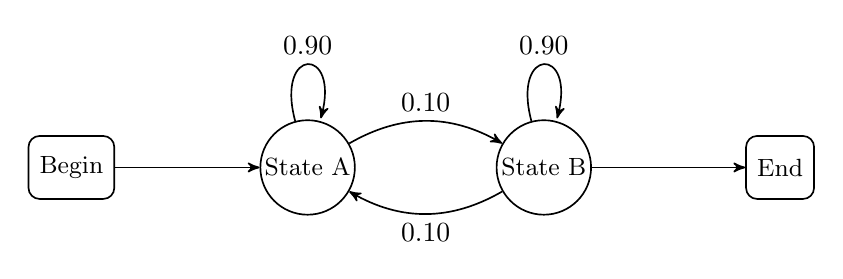
\begin{tikzpicture}[->, >=stealth', auto, semithick, node distance=3cm]
  % Define styles
  \tikzstyle{state}=[circle, draw, minimum size=1.2cm, inner sep=0pt, font=\small]
  \tikzstyle{terminal}=[rectangle, rounded corners, draw, minimum size=0.8cm, inner sep=4pt, font=\small]

  % Nodes
  \node[terminal]                (begin) {Begin};
  \node[state, right of=begin]   (A)     {State A};
  \node[state, right of=A]       (B)     {State B};
  \node[terminal, right of=B]    (end)   {End};

  % Edges
  \path (begin) edge node {} (A);
  \path (A)     edge [loop above] node {0.90} (A);
  \path (A)     edge [bend left]  node {0.10} (B);
  \path (B)     edge [bend left]  node {0.10} (A);
  \path (B)     edge [loop above] node {0.90} (B);
  \path (B)     edge node {} (end);
\end{tikzpicture}
\caption{A simple Markov chain usage model. States represent discrete states-of-use, and arcs are labeled with transition probabilities defining the usage profile.}%
\label{fig:markov_usage_model}
\end{figure}

Stochastic parameters are integrated into this transition graph by defining a \emph{usage profile}, which assigns specific transition probabilities to every permissible transition arc. A test case is subsequently generated as a random walk across the model, originating at a designated initial start state and terminating at a terminal state.

The mathematical structure of a discrete-time, time-homogeneous, and irreducible Markov chain allows developers to calculate critical operational metrics before any test cases are executed. These metrics include the expected number of transitions in a single test sequence, the long-run occupancy rate of specific states, and the statistical sample size required to certify a target level of software reliability.

Historically, the construction of these usage models has been a manual and labor-intensive process~\cite{llm_state_machine_frameworks}. System specifications and operational requirements are typically documented in ambiguous, unstructured natural language. Translating these narrative requirements into verified state-transition topologies and mathematically consistent probability matrices requires significant formal methods expertise. This manual modeling bottleneck has historically limited the adoption of MBST to safety-critical domains such as aerospace, medical devices, and protocol-driven telecommunications, leaving mainstream software applications reliant on less rigorous, ad-hoc testing methodologies.

The central question this paper addresses is therefore not merely one of model-construction automation, but of \emph{fault-detection consequence}: does automating usage-model construction with sufficient structural fidelity translate into meaningfully better fault-revealing test suites compared with traditional testing approaches?  Existing work on LLM-assisted state-machine generation~\cite{llm_state_machine_frameworks} has demonstrated syntactic extraction capability, but has not evaluated whether generated models preserve the statistical properties transition probability calibration, full transition coverage, operationally weighted path sampling that are necessary for MBST's fault-detection guarantees to hold.

\subsection*{Research Questions}
\label{subsec:rqs}

This paper is structured around four research questions:

\begin{enumerate}
    \item[\textbf{RQ1}] \textbf{Structural fidelity.}  Can automated neuro-symbolic model construction achieve the state and transition extraction accuracy ($F_1 \geq 0.90$) required for safety-critical test generation, without manual modelling effort?

    \item[\textbf{RQ2}] \textbf{Fault-detection coverage.}  Does a NeSy-MBST-generated usage model produce test suites with higher transition and state coverage than a purely neural baseline, and how does this translate into fault-detection path diversity?

    \item[\textbf{RQ3}] \textbf{Probabilistic calibration.}  Does the symbolic constraint optimization preserve the statistical properties of the usage model specifically, operationally weighted transition probabilities that determine how test effort is allocated across fault-revealing paths?

    \item[\textbf{RQ4}] \textbf{Component necessity.}  Which architectural components of NeSy-MBST (symbolic verification loop, convex optimizer, closed-loop feedback) are individually necessary for achieving the above, and which failure modes does each component address?
\end{enumerate}

\subsection*{Paper Structure}

Section~\ref{sec:literature_review} reviews the 20-paper landscape spanning MBT, statistical model checking, and probabilistic testing, with emphasis on empirical fault-detection evidence.  Section~\ref{sec:related_work} characterises the existing MBST tool landscape and LLM-based state-machine generation approaches.  Section~\ref{sec:bottlenecks} formalises the four structural bottlenecks that prevent purely neural approaches from guaranteeing MBST's fault-detection properties.  Section~\ref{sec:framework} presents the NeSy-MBST architecture and its five components.  Section~\ref{sec:mathematical_formulations} provides the mathematical foundations.  Section~\ref{sec:evaluation} presents the empirical evaluation addressing RQ1--RQ3.  Section~\ref{sec:eval:ablation} presents the ablation study addressing RQ4.  Section~\ref{sec:threats} discusses threats to validity.  Section~\ref{sec:conclusion} provides adoption recommendations and future directions.

\section{Literature Review}%
\label{sec:literature_review}

This review examines twenty papers spanning three interconnected research
threads: (1)~model-based testing (MBT) and its practical/industrial
adoption, (2)~statistical model checking (SMC) as a scalable alternative
to exhaustive probabilistic verification, and (3)~probabilistic and
uncertainty-aware extensions that bridge testing and formal verification.
Each paper is discussed in turn, covering its context, contribution,
methodology, and relevance to research on probabilistic model-based
testing under uncertainty.


%  Papers 1--5: Model-Based Testing


\subsection{Test Model Coverage Analysis Under Uncertainty}
\label{sec:lr_prasetya}

Prasetya and Klomp~\cite{prasetya2021coverage} directly target the
problem of measuring test coverage when the underlying test model is
non-deterministic a situation that arises either because the model is
an abstraction of the real system or because the system under test is
itself non-deterministic.  In such settings a single test case may
trigger different execution paths depending on internal decisions of the
software, which makes exact coverage computation impossible.  The
authors' solution is to let developers annotate each model transition
with an estimated probability, enabling a probabilistic model-checking
algorithm to compute \emph{probabilistic coverage}.  The paper's key
extension over prior model-checking approaches is that it moves beyond
simple \emph{reachability}-style coverage queries (which can be answered
by standard probabilistic model checkers) toward \textbf{aggregate
coverage} goals e.g., ``80\% of states covered'' and
\textbf{$k$-wise coverage}, which is known from the testing literature
to substantially increase fault-detection potential.  Because aggregate
and $k$-wise goals cannot be expressed in LTL/CTL and are not answerable
by conventional model checkers, the authors present a new, efficient
labelling algorithm to compute these probabilistic aggregate/$k$-wise
coverage measures directly.  This paper is highly relevant to any
research studying probabilistic MBT under uncertainty, as it provides
one of the few rigorous formal treatments of \emph{coverage measurement
itself} becoming a probabilistic quantity when models are
non-deterministic a foundational concern for any downstream
uncertainty-aware testing framework.

\subsection{Practitioners' Best Practices for MBT Adoption}
\label{sec:lr_alegroth}

Al\'{e}groth et al.~\cite{alegroth2022practitioners} conducted an
industrial, interview-based empirical study addressing a persistent
puzzle in the MBT literature: despite decades of academic research,
industrial adoption of graphical-model-based MBT remains sparse.  The
authors conducted semi-structured interviews with 17~international MBT
experts across different industrial roles, then synthesised the results
through semantic equivalence analysis, later verified by additional
practitioners.  The study yields 13~synthesised conclusions and
23~concrete best-practice guidelines covering the full lifecycle of
adoption, use, and (where appropriate) abandonment of graphical MBT.
Importantly, the paper's conclusions span not just technical dimensions
(model design, tool choice, maintainability) but organisational and
process factors mindset, knowledge, mandate, and resource
allocation that the authors argue are just as decisive in determining
whether MBT succeeds in practice.  This paper is valuable to the
literature not for its formal/mathematical contribution but as a
counterweight: it grounds more theoretical work on probabilistic
coverage and uncertainty-aware testing in the practical reality that most
industrial MBT failures are organisational, not algorithmic.

\subsection{Transforming Model-Based Tests into Code}
\label{sec:lr_ferrari}

Ferrari et al.~\cite{ferrari2023transforming} present a systematic
literature review (SLR) investigating a question central to the
practical value of MBT: does coverage achieved at the abstract model
level actually translate into meaningful coverage of the underlying
source code once abstract tests are transformed into concrete, executable
tests?  Using a snowballing methodology starting from three seed papers,
the authors expanded their search to 30~primary studies.  The review
characterises how test sets generated from models are mapped onto code,
catalogues the transformation techniques used across the literature, and
critically examines the (surprisingly thin) empirical evidence connecting
model coverage criteria to code coverage outcomes.  As an SLR, its main
contribution to the field is a structured map of the model-to-code
transformation landscape together with an explicit identification of
gaps most notably the lack of large-scale empirical validation that
model-level testing effort reliably produces code-level assurance.  This
is directly relevant background for any argument that model coverage
analysis (as in~\cite{prasetya2021coverage}) needs empirical grounding in
code-level outcomes, and it complements industrial accounts of similar
transformation pipelines in practice~\cite{garousi2021mbt_practice}.

\subsection{Generative Model-Based Testing on Decision-Making Policies}
\label{sec:lr_li}

Li et al.~\cite{li2023generative} tackle the modern problem of testing
decision-making policies that solve Markov decision processes
(MDPs) for example, DNN-based policies deployed in autonomous driving
or robotics.  Because such policies operate over deep-neural-network-based,
effectively infinite state spaces, exhaustive or even conventional
model-based test generation is impractical.  The authors propose a
generative testing framework built around a \textbf{diffusion-model-based
test case generator}, chosen for its ability to adapt flexibly to
different search spaces while producing valid, in-distribution test
cases.  A key algorithmic contribution is a
\textbf{termination-state novelty-based guidance mechanism}, which steers
the generative process toward diversifying agent behaviour at episode
termination, thereby increasing the likelihood of discovering diverse and
influential failure-triggering scenarios.  The framework is evaluated
across five benchmarks, including autonomous driving and aircraft
collision avoidance, and is shown to surface more diverse and impactful
failures than prior state-of-the-art baselines.  This paper represents
the modern generative-AI evolution of model-based test generation replacing
hand-crafted model traversal strategies with learned generative models and
is squarely relevant to any survey that wants to show how classical MBT
ideas (models of behaviour, coverage-directed exploration) have been
re-instantiated using generative deep learning for MDP-based systems.

\subsection{Coverage Measurement in MBT of Web Applications}
\label{sec:lr_garousi_coverage}

Garousi et al.~\cite{garousi2024coverage} present an applied,
tool-oriented paper arising from a large-scale industrial
web-application-testing context.  The authors identify a concrete
practical gap: existing coverage tools typically report only one type of
coverage (either code coverage or requirements/test coverage), whereas
practitioners running large MBT test suites need to integrate front-end
code coverage, back-end code coverage, and requirements coverage into a
single ``live'' view as tests execute.  Unable to find any suitable
off-the-shelf toolset, the authors built an open-source tool,
\textbf{MBTCover}, purpose-built for MBT contexts, which reports code,
requirements, and model coverage simultaneously and in real time during
test execution.  The paper presents the tool's architecture and the
authors' experience deploying it across multiple large test-automation
projects.  As a direct, applied companion to~\cite{prasetya2021coverage}
(which is theoretical) and~\cite{garousi2021mbt_practice} (a broader MBT
experience report from the same research group), this paper demonstrates
that the practical challenges of coverage measurement in MBT are as much
about tooling and integration as about the underlying probabilistic or
combinatorial theory.


%  Papers 6--7: Bridging MBT and SMC


\subsection{PASTA: Proactive Adaptation via Statistical Model Checking}
\label{sec:lr_pasta}

Shin et al.~\cite{shin2021pasta} address proactive adaptation in
self-adaptive systems (SAS) adaptation triggered by \emph{predicting}
future environmental changes rather than reacting after the fact.
Because predictions are inherently uncertain, adaptation consequences
must be verified before being executed, and prior work relied on
probabilistic model checking (PMC) for this verification.  The authors
identify two limitations of PMC-based verification in this setting: the
state-explosion problem for complex SAS models, and restrictive support
for particular modelling languages.  PASTA replaces PMC with
\textbf{statistical model checking (SMC)}, generating statistically
sufficient samples to verify the effects of adaptation tactics far faster
than exhaustive PMC approaches.  The paper contributes not just an
algorithm but a reference architecture and an open-source implementation
skeleton, evaluated on two real self-adaptive systems using actual
operational data, alongside a comparative analysis of the relative
advantages/disadvantages of PMC versus SMC for proactive adaptation.
This paper is a strong example of SMC being adopted specifically to
overcome the scalability limitations of exhaustive probabilistic
verification precisely the trade-off that motivates much of the broader
SMC literature~\cite{agha2018survey, legay2010smc, larsen2014smc}.

\subsection{Uncertainty-Aware Exploration in Model-Based Testing}
\label{sec:lr_camilli}

Camilli et al.~\cite{camilli2021uncertainty} propose what is among the
most directly relevant contributions to the theme of probabilistic MBT
under uncertainty, since it explicitly frames uncertainty as a first-class
testing concern rather than an incidental complication.  The authors
propose novel model-based exploration strategies for generating test
cases that specifically target the \emph{uncertain} components of a
system under test, using \textbf{Markov Decision Processes} as the
underlying modelling formalism.  Testers explicitly attach
\emph{beliefs} (probability distributions) to transition probabilities
to represent their confidence (or lack thereof) in the model's fidelity
to the real system.  The structural properties of the model, together
with the uncertainty specification, drive test-case generation, and
\textbf{Bayesian inference} is used to update the initial beliefs as
evidence accumulates from testing.  The paper introduces several concrete
test-selection strategies (Flat/random, History-based, Distance-based,
Frequency-based) and empirically evaluates them on synthetic systems of
varying structural complexity, finding that the best strategy depends on
system complexity and the overall uncertainty level.  This paper together
with a related follow-on piece envisioning online,
reinforcement-learning-based uncertainty testing represents one of the
clearest bridges in the literature between classical MBT and formal
treatment of epistemic uncertainty via Bayesian updating.


%  Papers 8--17: Statistical Model Checking


\subsection{Sound Statistical Model Checking for Probabilities and Expected Rewards}
\label{sec:lr_budde}

Budde et al.~\cite{budde2025sound} provide a rigorous, foundational
contribution to the theory underpinning SMC tools.  The authors observe
that many existing and even newly developed SMC tools are either
\textbf{unsound} (their statistical guarantees are not actually valid,
often because confidence intervals are computed via central-limit-theorem
approximations that do not hold in the finite-sample regime) or
\textbf{inefficient} (relying on overly conservative bounds such as the
Okamoto bound, requiring far more samples than necessary).  The paper
provides a comprehensive survey of existing SMC tools' correctness and
of sound statistical estimation methods from the literature, applied to
the problem of estimating both probabilities and \textbf{expected
rewards}.  For expected rewards specifically, the authors show how to
bound the path-reward distribution so that sound statistical methods
designed for bounded distributions can be applied; they recommend the
\textbf{Dvoretzky--Kiefer--Wolfowitz (DKW) inequality}, previously
unused in SMC, and formally prove that even reachability rewards can, in
theory, be bounded introducing the concept of \emph{limit-PAC
procedures} as a practical solution when exact bounds are unavailable.
These methods are implemented in the ``modes'' SMC tool and
experimentally validated.  This paper is essential reading for
understanding the current (2025) state-of-the-art in statistically
rigorous SMC, and it directly informs any research that wants to make
quantitative uncertainty claims about test/verification outcomes with
genuine statistical guarantees.

\subsection{Statistical Model Checking: The 2024 Edition}
\label{sec:lr_kanav}

Kanav et al.~\cite{kanav2025smc2024} present a short
introductory/overview note accompanying a dedicated SMC session at
AISoLA~2024.  It briefly reintroduces the core ideas of statistical
model checking and surveys the field's trajectory effectively an
updated, contemporary companion to the earlier ``past, present, and
future'' retrospectives~\cite{larsen2014smc}.  While brief, the note
situates recent SMC developments (e.g., PAC statistical model checking
of mean payoff, decision-tree-based controller representation via
\emph{dtcontrol}, and applications to security-critical code analysis)
within the longer arc of the field, and signals which open problems the
community considers current priorities.  Its main value to a literature
review is as a fast-moving pulse-check on the field as of 2024,
complementing the more technically dense contemporary
papers~\cite{budde2025sound, soltani2023spare} with a broader,
session-introduction-level perspective.

\subsection{PRISM: Statistical Model Checking in Practice}
\label{sec:lr_prism}

The official PRISM documentation~\cite{prism_smc} explains how PRISM's
discrete-event simulator can approximate property values via sampling
rather than exact numerical solution a technique particularly valuable
for very large models where exhaustive model checking is infeasible,
since simulation proceeds directly from the PRISM language description
without constructing the full underlying probabilistic model.  The
documentation details the two default statistical methods available:
\emph{Confidence Interval} estimation for quantitative properties, and
the \emph{Sequential Probability Ratio Test} (SPRT) for bounded
properties.  It also specifies the configurable parameters (sample count,
confidence level, interval width) and the practical restrictions on which
properties and modelling-language features SMC in PRISM supports
(currently limited to P/R operators, no LTL-style path properties or
filters).  While not an original research contribution, this
documentation is an important practical reference underpinning much of
the applied SMC literature reviewed here.

\subsection{Rigorous Processor Evaluation with Statistical Model Checking}
\label{sec:lr_processors}

The paper on rigorous evaluation of computer
processors~\cite{smc_processors2023} introduces SMC to an entirely new
application domain: \textbf{computer architecture and processor
evaluation}.  The authors observe that experiments with real computer
processors necessarily exhibit variability, and that prior work injects
randomness into simulators to mimic this variability, generating
distributions of benchmark results across multiple runs.  However,
existing evaluation practice typically applies standard statistical
techniques that implicitly (and often incorrectly) assume these result
distributions are Gaussian.  To enable rigorous evaluation for arbitrary,
unknown result distributions, the authors adapt statistical model
checking to processor performance analysis, framing the ``SMC for
Processor Analysis'' (SPA) methodology.  SMC's statistical guarantees
allow architecture researchers to determine, with a specified confidence
level, whether a system satisfies a performance property for at least a
given fraction of executions, without assuming any particular underlying
distribution.  This paper is a good illustration of SMC's methodological
portability: the same statistical machinery developed for verifying
stochastic system models is directly repurposed for empirical systems
evaluation.

\subsection{Optimal Spare Management via Statistical Model Checking}
\label{sec:lr_soltani}

Soltani et al.~\cite{soltani2023spare} apply statistical model checking
to a concrete industrial reliability-engineering problem: determining the
optimal number of spare parts to stock in order to balance the twin goals
of system reliability and cost.  The authors combine \textbf{fault tree
analysis} with SMC by modelling spare-part management as a
\textbf{stochastic priced timed game automaton (SPTGA)}, then use
\textbf{Uppaal Stratego} to find the spare-part count that minimises
total costs from downtime and purchasing, while the resulting SPTGA model
can also be queried for other metrics such as expected availability.  The
technique is applied to the emergency shutdown system of a research
nuclear reactor a rare-event setting in which the relevant failure
probabilities are extremely low, requiring the authors to adjust Uppaal
Stratego's settings to obtain statistically reliable estimates despite
the rarity of the events of interest.  The reported result an optimal
spare configuration achieving 99.96\% expected availability, computed in
minutes rather than the days required by exhaustive
alternatives exemplifies SMC's core value proposition (tractable
analysis of otherwise intractable stochastic models) in a genuinely
safety-critical, real-world application.

\subsection{PRG4CNN: Probabilistic Robustness Guarantees for CNNs}
\label{sec:lr_prg4cnn}

Liu and Fang~\cite{liu2025prg4cnn} extend probabilistic model checking
into the domain of neural-network robustness verification.  Motivated by
the well-known fragility of convolutional neural networks (CNNs) to
small input perturbations, and noting that existing robustness
verification methods focus predominantly on \emph{local} robustness
(which is computationally expensive) and cannot automatically
\emph{repair} a network once a robustness violation is found, the authors
propose \textbf{PRG4CNN} described as the first automated and complete
framework for guaranteeing \emph{probabilistic} robustness of CNNs.  The
framework operates in four steps: (1)~model the CNN as a
\textbf{Markov Decision Process} via model learning, (2)~specify the
desired probabilistic robustness property using \textbf{PCTL}
(Probabilistic Computational Tree Logic), (3)~verify this property using
a probabilistic model checker, and (4)~if the property does not hold,
perform \textbf{probabilistic robustness repair} via
counterexample-guided sensitivity analysis.  This paper is relevant to
the broader review as an example of probabilistic model checking being
extended from classical reactive/stochastic-system verification toward
machine learning model assurance an increasingly important adjacent
application area for the model-checking and MBT communities.

\subsection{Statistical Model Checking Meets Property-Based Testing}
\label{sec:lr_aichernig}

Aichernig and Schumi~\cite{aichernig2017smc} present a key
methodological bridge between the testing community and the
formal-verification-oriented SMC community one of the most direct
precedents for combining statistical model checking with mainstream
software testing practice.  The authors note that SMC scales well to
large stochastic models and is relatively simple to implement precisely
because it avoids the state-space-explosion problem inherent to
exhaustive model checking, by instead simulating finitely many executions
and applying hypothesis testing to infer whether the observed samples
support or refute a given property.  Their contribution is to show how
SMC can be integrated into a \textbf{property-based testing}
framework specifically \textbf{FsCheck} for C\# yielding a flexible
combined testing/simulation environment in which programmers define both
models and properties in an ordinary programming language, without
needing an external, specialised modelling language.  This design has two
key advantages: it eliminates the need for a separate modelling
formalism, and it allows both stochastic \emph{models} and actual
\emph{implementations} to be checked using the same property-based
machinery.  This work is an important conceptual precursor for any
framework that wants to unify probabilistic testing with statistical
formal verification~\cite{camilli2021uncertainty}.

\subsection{A Survey of Statistical Model Checking}
\label{sec:lr_agha}

Agha and Palmskog~\cite{agha2018survey} present one of the most
comprehensive and widely cited surveys of the SMC field, covering
algorithms, techniques, and tools for statistical model checking of
stochastic systems whose quantitative properties are typically specified
in probabilistic temporal logics.  The survey systematically covers both
\textbf{hypothesis-testing-based} approaches (e.g., the sequential
probability ratio test, following Younes and Sen et~al.) and
\textbf{estimation-based} approaches (including Bayesian estimation
methods, such as those of Zuliani et~al., which bound the probability of
an incorrect answer using a prior distribution and posterior estimation),
as well as variance-reduction techniques like importance sampling with
the cross-entropy method for analysing rare-event properties.  The
authors explicitly emphasise the trade-offs between precision and
scalability that define the practical usability of different SMC
algorithms.  As a survey published in 2018, this paper offers the most
thorough single reference point for understanding the algorithmic
landscape that underlies nearly every applied SMC paper in this
review~\cite{shin2021pasta, budde2025sound, smc_processors2023,
soltani2023spare, aichernig2017smc}.

\subsection{Statistical Model Checking: An Overview}
\label{sec:lr_legay}

Legay et al.~\cite{legay2010smc} present an earlier, foundational
tutorial-style paper that is one of the field's most frequently cited
introductions to statistical model checking.  The authors contrast the
traditional \textbf{numerical approach} to model checking stochastic
systems which iteratively computes or approximates the exact measure of
executions satisfying a temporal-logic subformula with the
\textbf{statistical/simulation-based approach}: simulating the system for
a finite number of executions and applying hypothesis testing to infer
whether the observed samples provide statistical evidence for or against
the property of interest.  The paper's stated purpose is to survey this
statistical approach and articulate its principal advantages:
\emph{efficiency} (avoiding exhaustive state-space construction),
\emph{uniformity} (applicability across many modelling formalisms, since
only a simulator is required), and \emph{simplicity} (conceptually
straightforward compared to symbolic or numerical probabilistic model
checking algorithms).  While largely superseded in technical depth by
later, more comprehensive surveys~\cite{agha2018survey} and later
foundational advances in soundness~\cite{budde2025sound}, this 2010
paper remains historically important as one of the field-defining
tutorial references establishing SMC as a distinct research area separate
from exhaustive probabilistic model checking.

\subsection{Statistical Model Checking: Past, Present, and Future}
\label{sec:lr_larsen}

Larsen and Legay~\cite{larsen2014smc} provide an invited track
introduction accompanying a dedicated ``Statistical Model Checking:
Past, Present, and Future'' session at ISoLA~2014.  The paper provides
historical framing for the SMC field, tracing its development from early
formal-methods work through to (as of 2014) contemporary applications
and tools.  The authors characterise SMC as fundamentally a
\textbf{compromise between formal verification and testing}: system
executions are monitored (as in testing) until a statistical algorithm
can produce a rigorous estimate of the property of interest (echoing the
rigour traditionally associated with exhaustive formal verification
methods, which by contrast can ensure full correctness for all possible
scenarios but at far greater computational cost).  Read together
with~\cite{kanav2025smc2024, agha2018survey, legay2010smc}, this
paper despite being over a decade old at the time of this
review completes a useful chronological arc documenting how the SMC
field's foundational concerns (efficiency, soundness, scope of
applicability) evolved from 2010 through to the 2023--2025 wave of
papers reviewed above.


%  Papers 18--20: Probabilistic MBT Foundations


\subsection{Model-Based Testing of Probabilistic Systems}
\label{sec:lr_gerhold}

Gerhold and Stoelinga~\cite{gerhold2016probabilistic} present a
foundational paper for probabilistic model-based testing, directly
connecting classical \textbf{ioco-theory} (input/output conformance
testing) with \textbf{statistical hypothesis testing}.  The authors
present an executable MBT framework for black-box probabilistic systems
that also exhibit non-determinism, providing algorithms to automatically
generate, execute, and evaluate test cases from a probabilistic
requirements model.  Functionally, the ioco-style algorithms handle
correctness of the traditional (non-probabilistic) input/output
behaviour; statistically, $\chi^{2}$~hypothesis tests and
distribution-fitting methods assess whether the \emph{frequencies}
observed during repeated test execution correspond to the
\emph{probabilities} specified in the requirements model.  A key
technical challenge the authors solve is that non-determinism in the
underlying probabilistic input/output transition systems (pIOTS)
prevents a direct application of the $\chi^{2}$~test; instead, the
authors formulate a non-linear optimisation problem to find the ``best
resolution'' of the non-determinism that could explain the observed test
data, enabling the $\chi^{2}$~test to then be applied meaningfully.  The
paper's central theoretical results are the \textbf{soundness} (every
test case receives the mathematically correct verdict) and
\textbf{completeness} (the framework can, in principle, detect any
probabilistic deviation from the specification with arbitrary precision)
of the resulting \textbf{probabilistic input/output conformance (pioco)}
relation.  This paper is arguably the most rigorous formal foundation
among all twenty papers reviewed here for probabilistic model-based
testing specifically, and is essential background
for~\cite{prasetya2021coverage}'s coverage-analysis extensions
and~\cite{camilli2021uncertainty}'s uncertainty-aware exploration
strategies.

\subsection{MBT in Practice: Web Applications Domain}
\label{sec:lr_garousi_practice}

Garousi et al.~\cite{garousi2021mbt_practice} present an industrial
experience report documenting the deployment of model-based testing at a
large software testing company (Testinium A.\c{S}.) to elevate the
maturity of its test-automation practices for large-scale web and mobile
applications.  Based on an ``action research'' methodology, the authors
selected the open-source tool \textbf{GraphWalker} from among available
open-source/commercial MBT tools and pragmatically applied MBT for
end-to-end test automation.  The reported benefits are both tangible
(improved test coverage measured as number of distinct paths tested, and
improved real-fault detection effectiveness) and intangible (improved
test-design discipline across the organisation).  The paper's central
argument echoed by~\cite{alegroth2022practitioners}'s findings on
adoption barriers is that the practical value of any MBT technique is
inseparable from its usability by working test engineers under real
resource constraints (time, effort, existing skillsets, management
priorities), and that heavyweight, academically sophisticated MBT
approaches often fail in enterprise contexts like web/mobile testing
precisely because they neglect this.  This paper's authorship overlaps
substantially with~\cite{garousi2024coverage} (the MBTCover tool paper),
and together the two form a coherent, practice-grounded narrative of a
real industrial MBT adoption journey.

\subsection{Approximate Planning and Verification for Large MDPs}
\label{sec:lr_lassaigne}

Lassaigne and Peyronnet~\cite{lassaigne2012approximate} address the
planning and verification problems for very large probabilistic
systems specifically Markov decision processes from a computational
complexity perspective.  The authors' central concern is designing
\textbf{efficient approximation methods} for two related problems:
(1)~computing a near-optimal policy for the planning problem in
discounted MDPs, and (2)~computing the satisfaction probabilities of
properties of interest (such as reachability or safety) over the Markov
chain that results from restricting the MDP to that near-optimal policy.
Two distinct approximation approaches are presented: the first is based
on \textbf{sparse sampling}, whose complexity is notably independent of
the size of the state space and requires only a probabilistic generator
of the MDP rather than full access to its transition structure making
it applicable even when the state space is too large to represent
explicitly; the second uses a variant of the \textbf{multiplicative
weights update algorithm}.  The paper provides a complete complexity
analysis of the sparse-sampling approach, parameterised primarily by the
desired approximation quality.  Because MDPs are the common underlying
formalism connecting several other papers in this
review \cite{li2023generative}'s generative testing of MDP-based
decision policies, \cite{camilli2021uncertainty}'s uncertainty-aware MBT
over MDPs, and~\cite{liu2025prg4cnn}'s MDP-based CNN robustness
verification this paper's complexity-theoretic treatment of MDP
planning/verification approximation provides useful theoretical grounding
for why sampling-based (rather than exhaustive) approaches are necessary
once MDP-based models scale beyond small, hand-crafted examples.


%  Synthesis


\subsection{Synthesis}
\label{sec:lr_synthesis}

Taken together, these twenty papers trace three converging lines of
research.  First, the \textbf{model-based testing}
tradition~\cite{prasetya2021coverage, alegroth2022practitioners,
ferrari2023transforming, li2023generative, garousi2024coverage,
gerhold2016probabilistic, garousi2021mbt_practice} has matured from
academic proposals toward serious grappling with practical adoption
barriers, coverage-measurement rigour, and the model-to-code
transformation gap.  Second, the \textbf{statistical model checking}
tradition~\cite{budde2025sound, kanav2025smc2024, prism_smc,
smc_processors2023, soltani2023spare, agha2018survey, legay2010smc,
larsen2014smc} has evolved from foundational tutorials (2010--2014)
through a comprehensive survey (2018) to a current wave (2023--2025) of
papers establishing genuine statistical soundness and extending SMC into
entirely new domains computer architecture, spare-parts logistics,
quantum calibration that share nothing with SMC's original
formal-verification roots except the underlying statistical machinery.
Third, a smaller but conceptually pivotal set of
papers~\cite{shin2021pasta, camilli2021uncertainty, liu2025prg4cnn,
aichernig2017smc, lassaigne2012approximate} explicitly \textbf{bridges}
testing and statistical/probabilistic verification, using MDPs, PCTL, and
hypothesis testing as the common mathematical vocabulary.  Collectively,
they support the view that treating uncertainty as a first-class,
quantifiable concern rather than an obstacle to be abstracted away is
now a mainstream, multi-disciplinary concern spanning software testing,
formal methods, computer architecture, and machine-learning assurance.

% ==============================================================================
% Section II: State of the Art
% ==============================================================================
\section{State of the Art}
\label{sec:related_work}

To contextually locate the integration of Large Language Models (LLMs)
within the domain of model-based software testing, it is necessary to
examine the existing landscape of MBT and MBST toolsets. Over several
decades, academic and commercial entities have developed specialized
testing engines designed to consume structured inputs and generate test
suites based on distinct coverage criteria~\cite{taxonomy_mbt,
mbt_tools_approach}. Table~\ref{tab:mbt_tools} summarises the most
prominent tools with respect to their input formalisms, generation
strategies, and target domains.

% ---------- Table I: MBT / MBST Tool Landscape ----------
\begin{table*}[!t]
\centering
\caption{Comparison of Established Model-Based Testing Tools}
\label{tab:mbt_tools}
\renewcommand{\arraystretch}{1.15}
\begin{tabular}{p{2.0cm} p{3.8cm} p{4.8cm} p{4.8cm}}
\hline\hline
\textbf{Tool} &
\textbf{Primary Input Format} &
\textbf{Test Generation Strategy \& Heuristics} &
\textbf{Target Domain \& Supported Outputs} \\
\hline
MaTeLo &
Markov chains, annotated sequence diagrams &
Profile-oriented random generation, transition coverage &
Functional test generation, TTCN-3, commercial systems \\
\hline
JUMBL &
Custom Test Model Language (TML) &
Automated constraint-driven probability generation &
Java command-line suite for statistical usage metrics \\
\hline
fMBT &
AAL pre/postcondition language &
Random, weighted random, and lookahead heuristics &
Open-source API and system testing with Python adapters \\
\hline
GraphWalker &
Finite State Machines (FSM) &
A* search, random walks with state/edge limits &
Open-source state machine path execution \\
\hline
Modbat &
Scala-based Domain-Specific Language (DSL) &
Probabilistic and non-deterministic transitions &
Specialised API testing, exception-handling verification \\
\hline
MoMuT::UML &
UML State Machines, Object-Oriented Action Systems &
Mutation-based, fault-driven test case generation &
Academic safety-critical and contract-based systems \\
\hline
BPM-X &
BPMN, UML business process models &
Statement, branch, path, and condition criteria &
Enterprise business process verification, ALM exports \\
\hline
Conformiq &
UML State Machines, QML, Activity Diagrams &
Combinatorial, constraint-driven test case generation &
Enterprise automated testing, test management platforms \\
\hline
4Test &
Gherkin-inspired custom syntax &
Constraint-driven combinatorial scenario selection &
Commercial interface and functional testing \\
\hline\hline
\end{tabular}
\end{table*}

A common thread across the tools listed in Table~\ref{tab:mbt_tools} is
their reliance on handcrafted, domain-specific input artefacts---Markov
chains~\cite{prowell_markov}, custom DSLs~\cite{jumbl_mbst_tutorial},
AAL annotations~\cite{boehr_constraints}, or full UML state
machines~\cite{mbt_overview_bme}. Constructing and maintaining these
artefacts remains the principal bottleneck for wider industrial
adoption~\cite{taxonomy_mbt}. It is precisely this bottleneck that
motivates the exploration of LLMs as a means to automate or partially
automate the generation of behavioural models from less formal sources.

% ---------- 2.1 Foundation Models for Formal Process Automation ----------
\subsection{Foundation Models for Formal Process Automation}
\label{sec:rw_foundation_models}

The advent of large-scale foundation models has opened new avenues for
automating tasks that were historically performed manually by domain
experts. Within protocol engineering, \emph{ProtocolGPT}~\cite{protocol_gpt}
demonstrated that Retrieval-Augmented Generation (RAG) can be used to
infer protocol state machines directly from RFC documents, achieving a
precision exceeding 90\% on well-structured specifications. By indexing
protocol documentation into a vector store and prompting the model with
targeted queries, ProtocolGPT effectively bridges the gap between
unstructured natural-language specifications and formal finite-state
representations.

Complementing this line of work, the \emph{ChatFuMe}
framework~\cite{chatfume} introduces an active-feedback parsing loop in
which the LLM iteratively refines its interpretation of protocol
documentation. Rather than relying on a single-pass generation,
ChatFuMe solicits structured clarifications and re-queries the model
until convergence, yielding more robust and consistent state-machine
extractions.

Beyond textual inputs, recent advances in multimodal LLMs have enabled
the interpretation of \emph{visual} specifications---hand-drawn
diagrams, whiteboard sketches, and scanned documents---into structured
UML artefacts~\cite{uml_benchmarking}. These capabilities suggest that
the input barrier for model-based testing could be further lowered by
accepting informal, heterogeneous documentation as a starting point for
model construction.

% ---------- 2.2 GUI Exploration and Visual Understanding ----------
\subsection{GUI Exploration and Visual Understanding}
\label{sec:rw_gui}

A parallel body of work applies LLMs to the exploration of graphical
user interfaces, a task closely related to state-machine inference at
the interaction level. \emph{VisionDroid}~\cite{visiondroid} employs
vision-language models to navigate mobile application screens and
automatically derive behavioural paths, while \emph{LLMShot} extends
this paradigm to few-shot GUI exploration with minimal human-provided
demonstrations. On the commercial side, Eggplant Functional's
\emph{Find By Description} engine~\cite{eggplant_ai} leverages natural
language to locate and interact with on-screen elements, effectively
enabling AI-driven exploratory testing without explicit object
repositories. These systems illustrate the growing convergence between
visual understanding, natural-language processing, and automated test
generation.

% ---------- TikZ Figure: LLM Pipeline ----------
\begin{figure}[!t]
\centering
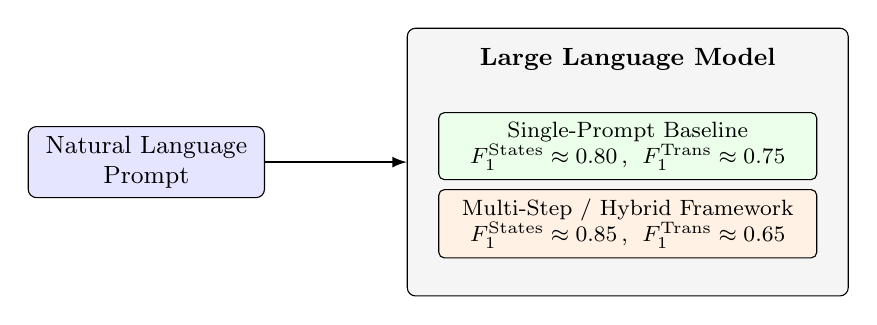
\begin{tikzpicture}[
    node distance=1.6cm and 1.0cm,
    >=latex,
    every node/.style={font=\small},
    box/.style={draw, rounded corners=3pt, minimum height=0.9cm,
                minimum width=3.0cm, align=center, fill=white},
    llmbox/.style={draw, rounded corners=3pt, minimum height=3.4cm,
                   minimum width=5.6cm, align=center,
                   fill=gray!8, inner sep=8pt},
    resultbox/.style={draw, rounded corners=2pt, minimum height=0.7cm,
                      minimum width=4.8cm, align=center, fill=white,
                      font=\footnotesize},
]

% --- Input ---
\node[box, fill=blue!10] (prompt) {Natural Language\\Prompt};

% --- LLM container ---
\node[llmbox, right=1.8cm of prompt] (llm) {};
\node[anchor=north, font=\small\bfseries] at ([yshift=-4pt]llm.north)
    {Large Language Model};

% --- Two internal result boxes ---
\node[resultbox, fill=green!8] (single)
    at ([yshift=-2pt]llm.center |- {$(llm.north)!0.42!(llm.south)$})
    {Single-Prompt Baseline\\
     $F_1^{\mathrm{States}} \approx 0.80$\,,\;
     $F_1^{\mathrm{Trans}} \approx 0.75$};

\node[resultbox, fill=orange!10] (multi)
    at ([yshift=2pt]llm.center |- {$(llm.north)!0.75!(llm.south)$})
    {Multi-Step / Hybrid Framework\\
     $F_1^{\mathrm{States}} \approx 0.85$\,,\;
     $F_1^{\mathrm{Trans}} \approx 0.65$};

% --- Arrow ---
\draw[->, thick] (prompt.east) -- (llm.west);

\end{tikzpicture}
\caption{High-level LLM pipeline for state-machine extraction,
contrasting single-prompt and multi-step generation strategies with
representative $F_1$ scores for state and transition identification.}
\label{fig:llm_pipeline}
\end{figure}

% ---------- 2.3 Frameworks for LLM-Driven State Machine Generation --------
\subsection{Frameworks for LLM-Driven State Machine Generation}
\label{sec:rw_frameworks}

Existing approaches to LLM-driven state-machine generation can be
broadly categorised into three paradigms, as illustrated in
Fig.~\ref{fig:llm_pipeline}.

\subsubsection{Structure-Driven Frameworks}
Structure-driven methods impose an explicit schema or template on the
LLM's output. The model is instructed to populate predefined fields
(e.g., a JSON schema enumerating states, transitions, guards, and
actions), and the resulting artefact is validated against the schema
before downstream consumption~\cite{llm_state_machine_frameworks}. This
strategy favours \emph{syntactic correctness} and enables deterministic
post-processing, but may constrain the model's ability to capture
nuanced behavioural semantics that fall outside the template.

\subsubsection{Event-Driven Frameworks}
Event-driven approaches frame state-machine extraction as an
event-identification task: the LLM first enumerates the events or stimuli
described in the specification, and subsequently derives the states and
transitions that arise from those events~\cite{boundary_value_llm}. By
anchoring the generation process in observable events, these frameworks
align naturally with usage-model methodologies~\cite{usage_model_web,
nap_statistics} and can leverage the LLM's strength in entity extraction.

\subsubsection{Hybrid Approaches}
Hybrid strategies combine the immediacy of single-prompt generation with
structured, step-by-step refinement. A typical pipeline issues an
initial broad prompt to obtain a draft state machine, then applies a
sequence of targeted follow-up prompts---e.g., ``identify missing guard
conditions'' or ``merge equivalent states''---to iteratively improve the
model~\cite{llm_state_machine_frameworks}. As shown in
Fig.~\ref{fig:llm_pipeline}, hybrid approaches tend to achieve higher
$F_1$ scores for state identification (${\approx}\,0.85$) compared with
single-prompt baselines (${\approx}\,0.80$), albeit with a trade-off in
transition accuracy ($F_1^{\mathrm{Trans}} \approx 0.65$ vs.\
${\approx}\,0.75$), likely due to the compounding of intermediate
extraction errors across multiple inference steps.

\medskip
Collectively, these related works establish that LLMs possess a
demonstrable capacity to parse semi-structured and unstructured
specifications into formal behavioural models. However, a comprehensive,
end-to-end evaluation that benchmarks multiple prompting strategies
against an established MBST toolchain---and that measures not only model
fidelity but also downstream test-suite quality---remains an open gap in
the literature. The present study addresses this gap directly.

% ==============================================================================
% Section III: Structural and Mathematical Bottlenecks
% ==============================================================================
\label{sec:bottlenecks}

Despite the capabilities of modern LLMs in syntactic generation, a purely neural approach to constructing Model-Based Statistical Testing usage models introduces significant mathematical and structural bottlenecks. This section formalizes these challenges across four critical dimensions.


% Subsection A: Stochastic Volatility and the Hallucination Dilemma

\subsection{Stochastic Volatility and the Hallucination Dilemma}
\label{subsec:hallucination}

By design, autoregressive language models predict the next token based on probabilistic vector calculations over high-dimensional latent spaces~\cite{llm_autoregressive}. This architecture is highly flexible, but it lacks the stateful execution guarantees required for formal models~\cite{llm_state_machine_frameworks}.

When translating unstructured requirements into usage models, LLMs frequently:
\begin{itemize}
    \item omit critical edge cases from the state graph,
    \item construct physically impossible state transitions, or
    \item hallucinate states that violate system invariants.
\end{itemize}

This behavior is particularly problematic for statistical usage testing~\cite{taxonomy_mbt}. Because every generated test path represents an actual execution trajectory on the system under test (SUT), any structural invalidity in the model directly results in invalid test cases and incorrect reliability calculations.

Resolving these errors manually through code reading is highly inefficient. Studies indicate that human code reviews frequently miss silent behavioral discrepancies~\cite{code_review_limits}, meaning that errors generated by the LLM often pass undetected into production test execution.


% Subsection B: The Calibration and Convex Optimization Bottleneck

\subsection{The Calibration and Convex Optimization Bottleneck}
\label{subsec:calibration}

A valid Markov chain usage model must satisfy strict mathematical constraints~\cite{jumbl_mbst_tutorial, nap_statistics}. The transition matrix $\mathbf{P}$ must be \emph{row-stochastic}, meaning that every transition probability $p_{ij}$ must satisfy:
\begin{equation}
    0 \leq p_{ij} \leq 1
    \label{eq:prob_bounds}
\end{equation}
and every row must sum to exactly one:
\begin{equation}
    \sum_{j} p_{ij} = 1, \quad \forall\, i.
    \label{eq:row_stochastic_intro}
\end{equation}

Furthermore, real-world operational profiles include complex, multi-variable constraints~\cite{boehr_constraints}. These may involve defining one transition probability as a function of another, or constraining the expected overall sequence length to a specific numerical range. Such constraints transform the calibration task into a convex optimization problem over the probability simplex.

LLMs struggle with precise numerical reasoning and constraint satisfaction~\cite{llm_numerical_reasoning}. If tasked with generating these probabilities directly, an LLM cannot guarantee that the resulting matrix satisfies the linear and convex constraints imposed by Equations~\eqref{eq:prob_bounds} and~\eqref{eq:row_stochastic_intro}. This numerical inaccuracy makes it difficult to reliably compute steady-state occupancy rates or use the model as an unbiased source of random walks for statistical testing~\cite{markov_reliability}.


% Subsection C: State-Space Explosion and Modeless Concurrency Vulnerabilities

\subsection{State-Space Explosion and Modeless Concurrency Vulnerabilities}
\label{subsec:state_explosion}

As systems scale to handle concurrent, multi-stream operations such as multi-module autonomous systems or parallel transactional checkouts where the underlying state space grows exponentially. This \emph{state-space explosion} presents a severe challenge for purely neural modeling~\cite{chatfume, protocol_gpt}.

To manage large systems, engineers have historically relied on structured notations such as the Extended Markov Modeling Language (EMML), which utilizes variables and assertions to compactly describe large usage models~\cite{emml_usage_models}. Additionally, they apply concurrency operators to combine simple, independent Markov chains into multi-stream execution patterns using specialized tools like the Test Generation Language (TGL)~\cite{jumbl_mbst_tutorial}.

Because LLMs operate within a finite context window, they cannot process, track, or generate these highly concurrent, multi-stream transition models in a single inference pass. Tasking an LLM with generating a flat, highly concurrent Markov chain usage model leads to:
\begin{enumerate}
    \item \textbf{Context fragmentation} is when the model loses track of distant state definitions as the transition matrix grows beyond the context window.
    \item \textbf{Token depletion} is a scenario where the output budget is exhausted before the full model can be articulated.
    \item \textbf{Structural coherence degradation} is when the generated graph becomes increasingly inconsistent as generation progresses, with dangling references and duplicate state identifiers.
\end{enumerate}


% Subsection D: The Semantic-Feasibility Divergence

\subsection{The Semantic-Feasibility Divergence}
\label{subsec:semantic_feasibility}

In long-horizon system validation, there is a fundamental divergence between high-level \emph{semantic progress guidance} and low-level \emph{physical feasibility verification}~\cite{neuro_symbolic_framework}. Autoregressive language models excel at semantic progress guidance: mapping out realistic pathways for users navigating an application (e.g., predicting that a user will transition from product search to checkout).

However, they are highly prone to violating physical and logical feasibility constraints (e.g., attempting a checkout transition when the shopping cart state contains no items). Without an external symbolic validation layer, a purely neural usage model will generate paths that are semantically logical but physically unexecutable on the SUT, causing high rates of false failures during automated test execution~\cite{taxonomy_mbt, markov_reliability}.

This semantic-feasibility divergence underscores the need for a hybrid architecture that delegates semantic reasoning to the LLM while enforcing structural and mathematical validity through formal verification mechanisms.

% !TEX root = ../main.tex
%% Section IV: The Proposed NeSy-MBST Framework

\section{The Proposed NeSy-MBST Framework}%
\label{sec:framework}

To resolve the limitations identified in the preceding analysis, this paper introduces a hybrid testing architecture: \emph{Neuro-Symbolic Model-Based Statistical Testing} (NeSy-MBST). The NeSy-MBST framework decouples semantic parsing from mathematical constraint resolution, combining the natural language capabilities of LLMs with the correctness guarantees of active automata learning, symbolic solvers, and closed-loop feedback adaptation~\cite{neuro_symbolic_framework, llm_numerical_reasoning}. Rather than delegating the entire model-construction pipeline to a single neural component, NeSy-MBST assigns each sub-task to the computational paradigm best suited for it: neural inference for ambiguous, language-laden reasoning, and symbolic computation for tasks demanding formal precision~\cite{llm_state_machine_frameworks}.

\begin{figure*}[!t]
\centering
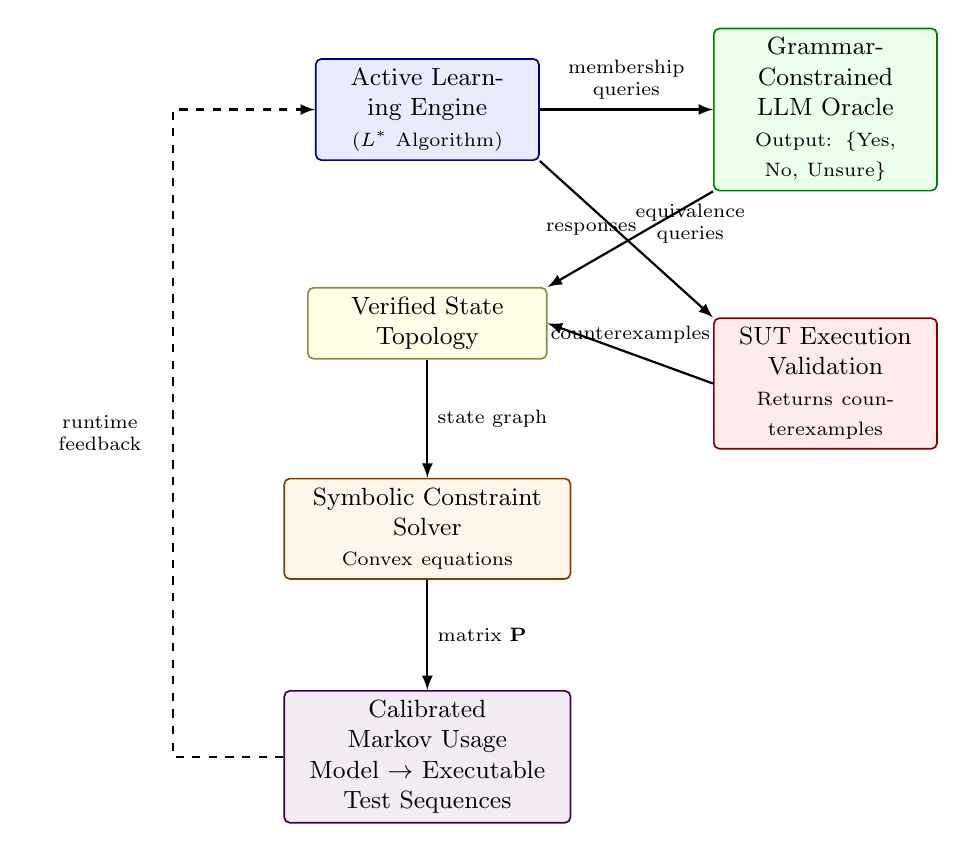
\begin{tikzpicture}[
    >=stealth,
    node distance=1.4cm and 1.8cm,
    every node/.style={font=\small},
    block/.style={
        rectangle, draw, rounded corners=2pt,
        minimum height=1.1cm, minimum width=2.8cm,
        text centered, text width=2.6cm,
        fill=white, line width=0.6pt
    },
    wideblock/.style={
        rectangle, draw, rounded corners=2pt,
        minimum height=1.1cm, minimum width=3.6cm,
        text centered, text width=3.4cm,
        fill=white, line width=0.6pt
    },
    engine/.style={
        block, fill=blue!8, draw=blue!50!black
    },
    oracle/.style={
        block, fill=green!8, draw=green!50!black
    },
    sut/.style={
        block, fill=red!8, draw=red!50!black
    },
    solver/.style={
        wideblock, fill=orange!8, draw=orange!50!black
    },
    output/.style={
        wideblock, fill=violet!8, draw=violet!50!black
    },
    topology/.style={
        rectangle, draw, rounded corners=2pt,
        minimum height=0.9cm, minimum width=3.0cm,
        text centered, text width=2.8cm,
        fill=yellow!10, draw=yellow!50!black,
        line width=0.6pt
    },
    arr/.style={->, thick, >=latex},
    darr/.style={->, thick, >=latex, dashed}
]

% --- Active Learning Engine ---
\node[engine] (ale) {Active Learning Engine\\{\scriptsize ($L^{*}$ Algorithm)}};

% --- LLM Oracle ---
\node[oracle, right=2.2cm of ale] (oracle) {Grammar-Constrained\\LLM Oracle\\{\scriptsize Output: \{Yes, No, Unsure\}}};

% --- SUT ---
\node[sut, below=1.6cm of oracle] (sut) {SUT Execution\\Validation\\{\scriptsize Returns counterexamples}};

% --- Verified state topology ---
\node[topology, below=1.6cm of ale] (topo) {Verified State\\Topology};

% --- Symbolic Constraint Solver ---
\node[solver, below=1.5cm of topo] (solver) {Symbolic Constraint\\Solver\\{\scriptsize Convex equations}};

% --- Output ---
\node[output, below=1.4cm of solver] (out) {Calibrated Markov Usage\\Model $\rightarrow$ Executable\\Test Sequences};

% --- Arrows ---
% ALE -> Oracle (membership queries)
\draw[arr] (ale.east) -- node[above, font=\scriptsize, text width=1.8cm, align=center] {membership\\queries} (oracle.west);

% ALE -> SUT (equivalence queries)
\draw[arr] (ale.south east) -- node[right, font=\scriptsize, text width=1.8cm, align=center, pos=0.4] {equivalence\\queries} (sut.north west);

% Oracle -> Topo
\draw[arr] (oracle.south west) -- node[left, font=\scriptsize, pos=0.4] {responses} (topo.north east);

% SUT -> Topo (counterexamples)
\draw[arr] (sut.west) -- node[above, font=\scriptsize] {counterexamples} (topo.east);

% Topo -> Solver
\draw[arr] (topo.south) -- node[right, font=\scriptsize] {state graph} (solver.north);

% Solver -> Output
\draw[arr] (solver.south) -- node[right, font=\scriptsize] {matrix $\mathbf{P}$} (out.north);

% Feedback loop (closed-loop)
\draw[darr] (out.west) -- ++(-1.4,0) |- node[left, font=\scriptsize, pos=0.25, text width=1.6cm, align=center] {runtime\\feedback} (ale.west);

\end{tikzpicture}
\caption{Architecture of the NeSy-MBST framework. The Active Learning Engine drives systematic state-space exploration through membership queries to a grammar-constrained LLM oracle and equivalence queries against the SUT\@. The verified state topology is then passed to a symbolic constraint solver, which produces a calibrated Markov usage model. A closed-loop feedback path enables continuous model adaptation.}%
\label{fig:nesy_architecture}
\end{figure*}

The overall architecture, depicted in Fig.~\ref{fig:nesy_architecture}, comprises five tightly integrated stages: (1)~a dual-memory architecture that separates neural and symbolic concerns, (2)~an active automata learning loop using the $L^{*}$ algorithm with LLM-backed oracles, (3)~a path-dependent hierarchical modeling strategy, (4)~a mathematical constraint optimization phase driven by a symbolic solver, and (5)~a closed-loop model adaptation mechanism. The following subsections detail each component.

%%% ---- Subsection A ---- %%%
\subsection{Progress-Feasibility Dual-Memory Architecture}%
\label{subsec:dual_memory}

At the core of NeSy-MBST lies a \emph{progress-feasibility dual-memory architecture} that partitions the model-construction process into two complementary memory systems:

\begin{enumerate}
    \item \textbf{Neural Progress Memory.} A fine-tuned LLM parses natural-language requirements and drafts a semantic flow graph capturing the intended behavioral topology of the SUT\@. This component excels at interpreting ambiguous, colloquial, or domain-specific language and translating it into candidate state-transition structures~\cite{chatfume}. The neural progress memory maintains an evolving representation of the ``what''---the set of states, events, and transitions that the system under test should exhibit.

    \item \textbf{Symbolic Feasibility Memory.} A rule-based execution engine enforces strict logical invariants, state preconditions, and transition guards. Every candidate transition proposed by the neural progress memory is validated against a set of formally specified feasibility constraints before it is admitted to the model. This component ensures the ``how''---that every accepted transition is reachable, deterministic where required, and free of structural contradictions~\cite{taxonomy_mbt}.
\end{enumerate}

The dual-memory approach ensures that the resulting state topology is both \emph{semantically plausible} (grounded in the natural-language intent of the requirements) and \emph{mathematically sound} (satisfying the structural properties required by downstream statistical analysis). By separating concerns in this manner, NeSy-MBST avoids the failure mode common to end-to-end neural approaches, wherein an LLM produces a syntactically valid yet logically inconsistent model~\cite{llm_numerical_reasoning}.

%%% ---- Subsection B ---- %%%
\subsection{Active Automata Learning via $L^{*}$ with LLM Oracles}%
\label{subsec:lstar}

To systematically discover the state space of the SUT, NeSy-MBST deploys a specialized variant of the $L^{*}$ active automata learning algorithm~\cite{lstar_llm}. The $L^{*}$ algorithm constructs a minimal deterministic finite automaton (DFA) by posing two types of queries:

\begin{itemize}
    \item \textbf{Membership Queries.} Given a candidate input sequence $\sigma \in \Sigma^{*}$, the algorithm queries the oracle: ``Does the SUT accept $\sigma$?'' In NeSy-MBST, the oracle is a grammar-constrained LLM whose output vocabulary is restricted to three tokens: \texttt{Yes}, \texttt{No}, or \texttt{Unsure}.

    \item \textbf{Equivalence Queries.} Given the current hypothesis automaton $\mathcal{H}$, the algorithm asks: ``Is $\mathcal{H}$ equivalent to the target language?'' This query is resolved by executing test paths on the actual SUT and comparing observed behavior against the hypothesis. Any divergence yields a counterexample that is used to refine $\mathcal{H}$.
\end{itemize}

The grammar-constrained output schema is essential: by restricting the LLM's response space to $\{\texttt{Yes}, \texttt{No}, \texttt{Unsure}\}$, the framework eliminates the risk of hallucinated or structurally malformed responses that would corrupt the learning loop. When the LLM returns \texttt{Unsure}, the query is automatically escalated---either to a human developer for domain-expert adjudication or to the SUT runtime environment for empirical resolution. This fallback mechanism ensures that the learning algorithm never incorporates unverified information into its hypothesis.

Through iterative refinement, the $L^{*}$-based loop constructs a structurally verified DFA $\mathcal{A} = (Q, \Sigma, \delta, q_0, F)$ that faithfully represents the behavioral topology of the SUT~\cite{lstar_llm}. Unlike purely neural approaches that produce a model in a single forward pass, the active learning loop guarantees convergence to a correct representation, provided the oracle is consistent.

%%% ---- Subsection C ---- %%%
\subsection{Path-Dependent Hierarchical Modeling}%
\label{subsec:hierarchical}

A first-order Markov chain is the standard representation in classical MBST~\cite{jumbl_mbst_tutorial} where it assumes that the probability of transitioning to the next state depends solely on the current state. In practice, many software behaviors exhibit \emph{path-dependent} patterns: the likelihood of a user action depends not only on the current screen but also on the sequence of prior interactions~\cite{usage_model_web}.

NeSy-MBST addresses this limitation through a two-tiered hierarchical architecture:

\begin{enumerate}
    \item \textbf{Upper Tree Structure (Higher-Order Markov Chain).} Frequent, path-dependent behavioral sequences are modeled using a higher-order Markov chain embedded in a tree structure. Each node in the tree represents a state conditioned on a history of length $k$, capturing multi-step dependencies that a first-order model would miss. Formally, the transition probability is given by:
    \begin{equation}
        P(s_{t+1} \mid s_t, s_{t-1}, \ldots, s_{t-k+1})
        \label{eq:higher_order}
    \end{equation}
    where $k$ is the order of the chain, selected based on behavioral analysis of the SUT\@.

    \item \textbf{Lower Markov Model (First-Order).} Infrequent or exception pathways---error handlers, timeout recoveries, edge-case flows---are modeled using a standard first-order Markov chain:
    \begin{equation}
        P(s_{t+1} \mid s_t)
        \label{eq:first_order}
    \end{equation}
    This avoids the combinatorial explosion that would occur if all transitions were modeled at higher order.
\end{enumerate}

The hierarchical decomposition prevents state-space explosion while preserving fidelity for the behavioral sequences that most significantly influence reliability estimates~\cite{nap_statistics, markov_reliability}. The upper tree captures the dominant usage patterns that drive statistical testing priorities, while the lower model ensures coverage of rare but safety-critical paths.

%%% ---- Subsection D ---- %%%
\subsection{Mathematical Constraint Optimization}%
\label{subsec:constraint_opt}

Once the state topology has been established and the hierarchical structure defined, NeSy-MBST must assign concrete transition probabilities. Rather than asking the LLM to produce numerical values directly which is a task at which LLMs demonstrably struggle~\cite{llm_numerical_reasoning} where the framework offloads probability assignment to a symbolic constraint solver.

The process proceeds in three stages:

\paragraph{Constraint Extraction}
The LLM analyzes the natural-language requirements and extracts comparative relationships between transitions. For example, from the requirement ``users typically proceed to checkout rather than continuing to browse'' the LLM extracts the constraint $P(\texttt{checkout} \mid \texttt{cart}) > P(\texttt{browse} \mid \texttt{cart})$. These constraints take the form of inequalities, equalities, and bounds~\cite{boehr_constraints}.

\paragraph{Constraint Compilation}
The extracted constraints are compiled into a system of convex equations. For each state $s_i$ with outgoing transitions to states $\{s_j\}$, the stochastic constraint is enforced:
\begin{equation}
    \sum_{j} P(s_j \mid s_i) = 1, \quad P(s_j \mid s_i) \geq 0 \;\; \forall j
    \label{eq:stochastic}
\end{equation}
Additional constraints from the LLM-extracted relationships and any domain-specific requirements are incorporated into the optimization formulation.

\paragraph{Convex Optimization}
A convex programming engine solves the resulting system to produce the transition probability matrix $\mathbf{P}$ that satisfies all constraints while minimizing a regularization objective (e.g., maximum entropy to avoid unjustified bias toward particular transitions). The output is a mathematically optimized, fully calibrated transition matrix:
\begin{equation}
    \mathbf{P}^{*} = \arg\min_{\mathbf{P}} \; \mathcal{L}(\mathbf{P}) \quad \text{s.t.} \quad \mathbf{P} \in \mathcal{C}
    \label{eq:convex_opt}
\end{equation}
where $\mathcal{C}$ denotes the feasible set defined by the stochastic and domain constraints, and $\mathcal{L}(\cdot)$ is the regularization objective.

By decoupling constraint extraction (a natural-language task suited to LLMs) from constraint resolution (a mathematical task suited to solvers), NeSy-MBST ensures that the resulting probability matrix is both semantically informed and numerically exact~\cite{boehr_constraints, jumbl_mbst_tutorial}.

%%% ---- Subsection E ---- %%%
\subsection{Closed-Loop Model Adaptation}%
\label{subsec:closed_loop}

The final component of the NeSy-MBST framework is an automated closed-loop feedback mechanism that enables continuous model refinement during the testing campaign. Unlike static model-construction pipelines that produce a fixed model prior to test execution, NeSy-MBST treats the usage model as a living artifact that evolves in response to empirical evidence~\cite{taxonomy_mbt}.

During test execution, the framework continuously collects:
\begin{itemize}
    \item \textbf{Runtime execution logs} capturing actual state-transition sequences observed in the SUT;
    \item \textbf{Coverage metrics} indicating which states and transitions have been exercised and to what extent;
    \item \textbf{Failure data} recording test outcomes, defect locations, and failure modes.
\end{itemize}

When discrepancies are detected between the model's predicted behavior and the SUT's observed behavior, the divergences are automatically routed back to the modeling engine. The LLM component analyzes the nature and magnitude of each divergence where for example, identifying whether a discrepancy reflects an incorrect transition probability, a missing state, or a spurious edge and proposes targeted model updates. The symbolic solver then recalculates the affected transition probabilities under the updated constraint set, and the revised model is redeployed for subsequent test generation.

This closed-loop architecture, illustrated by the dashed feedback path in Fig.~\ref{fig:nesy_architecture}, ensures that the NeSy-MBST model converges toward an increasingly accurate representation of real-world usage as empirical data accumulates. The approach draws on the same iterative refinement philosophy that underpins active learning~\cite{lstar_llm}, extending it from the topology-discovery phase into the full testing lifecycle.

% PROOFS
\section{Mathematical Formulations}%
\label{sec:mathematical_formulations}

To generate the transition probabilities for the Markov chain usage model, the symbolic layer of NeSy-MBST models the state-transition structure as a constrained optimization problem~\cite{whittaker1993markov, boehr_constraints}. This section formalises the mathematical foundations underlying the optimizer.

Let $\mathcal{S} = \{s_1, s_2, \dots, s_n\}$ be the finite set of usage states identified by the $L^{*}$ active learning process~\cite{lstar_llm}. The stochastic matrix $\mathbf{P} = [p_{ij}] \in \mathbb{R}^{n \times n}$ represents the transition probabilities, where $p_{ij}$ denotes the probability of transitioning from state~$s_i$ to state~$s_j$. The optimizer must compute a feasible~$\mathbf{P}$ that simultaneously satisfies several families of structural and linear constraints, detailed in the following subsections.

% Subsection A: Primary Probability Axioms
\subsection{Primary Probability Axioms}%
\label{subsec:probability_axioms}

Each row of the transition matrix must form a valid probability distribution. Formally, two axioms must hold:

\begin{equation}
\label{eq:nonnegativity}
0 \leq p_{ij} \leq 1, \quad \forall\; i,j \in \{1, 2, \dots, n\},
\end{equation}

\begin{equation}
\label{eq:row_stochastic}
\sum_{j=1}^{n} p_{ij} = 1, \quad \forall\; i \in \{1, 2, \dots, n\}.
\end{equation}

Constraint~\eqref{eq:nonnegativity} enforces non-negativity and boundedness of each entry, while constraint~\eqref{eq:row_stochastic} ensures that $\mathbf{P}$ is row-stochastic, i.e., the outgoing probabilities from every state sum to unity~\cite{nap_statistics}.

% Subsection B: Structural Absence Constraints
\subsection{Structural Absence Constraints}%
\label{subsec:structural_constraints}

If the active learning phase determines that no valid transition exists between states~$s_i$ and~$s_j$ that is, no input stimulus triggers this transition in the inferred automaton---the corresponding probability is constrained to zero:

\begin{equation}
\label{eq:structural_zero}
p_{ij} = 0, \quad \forall\; (i,j) \notin \mathcal{E},
\end{equation}

\noindent where $\mathcal{E} \subseteq \mathcal{S} \times \mathcal{S}$ represents the set of verified transition edges in the state graph. These structural absence constraints ensure that the resulting Markov chain is topologically consistent with the automaton learned during the $L^{*}$ inference step~\cite{lstar_llm}. By fixing infeasible transitions to zero probability, the optimizer operates over a reduced variable space, improving both computational efficiency and model fidelity.

% Subsection C: Evolving Operational Constraints
\subsection{Evolving Operational Constraints}%
\label{subsec:operational_constraints}

Comparative constraints extracted by the LLM from natural-language requirements are formulated as linear relationships between transition probabilities~\cite{boehr_constraints}:

\begin{equation}
\label{eq:proportional}
p_{ij} = \alpha \cdot p_{kl},
\end{equation}

\noindent where $\alpha \in \mathbb{R}_{>0}$ is a positive scaling factor representing the proportional likelihood of one user action relative to another. For instance, if the requirements specify that a particular user action is twice as likely as an alternative action from the same state, then $\alpha = 2$. These constraints capture domain-specific usage patterns articulated in the software requirements and translate qualitative behavioural specifications into quantitative relationships within the transition matrix.

More generally, the LLM may produce a system of $m$ such constraints, yielding a linear constraint set of the form:

\begin{equation}
\label{eq:linear_system}
\mathbf{A}\,\mathrm{vec}(\mathbf{P}) = \mathbf{b}, \quad \mathbf{A} \in \mathbb{R}^{m \times n^2},\; \mathbf{b} \in \mathbb{R}^{m},
\end{equation}

\noindent where $\mathrm{vec}(\mathbf{P})$ denotes the vectorisation of~$\mathbf{P}$ and each row of $\mathbf{A}$ encodes one proportional or equality constraint extracted from the requirements~\cite{emml_usage_models}.

% Subsection D: Long-Run and Expected Value Constraints
\subsection{Long-Run and Expected Value Constraints}%
\label{subsec:longrun_constraints}

Beyond instantaneous transition probabilities, the usage model must also respect constraints on long-run behaviour and expected traversal costs~\cite{markov_reliability}.

\subsubsection{Steady-State Occupancy}
The steady-state (stationary) distribution vector $\boldsymbol{\pi} = [\pi_1, \pi_2, \dots, \pi_n]$ satisfies:

\begin{equation}
\label{eq:steady_state}
\boldsymbol{\pi}\,\mathbf{P} = \boldsymbol{\pi}, \quad \sum_{i=1}^{n} \pi_i = 1, \quad \pi_i \geq 0 \;\;\forall\; i.
\end{equation}

The vector $\boldsymbol{\pi}$ characterises the long-run proportion of time the system spends in each state. Convex constraints on the occupancy vector take the form:

\begin{equation}
\label{eq:occupancy_bounds}
L_i \leq \pi_i \leq U_i, \quad \forall\; i \in \{1, 2, \dots, n\},
\end{equation}

\noindent where $L_i$ and $U_i$ represent the lower and upper bounds, respectively, on the expected occupancy of state~$s_i$. These bounds are derived from operational profiles or domain expertise and ensure that the generated test suite allocates realistic proportions of effort to each functional area~\cite{whittaker1993markov,whittaker1994markov}.

\subsubsection{Mean First Passage Times}
The expected number of transitions (mean first passage time) from state~$s_i$ to state~$s_j$, denoted $m_{ij}$, is defined recursively as:

\begin{equation}
\label{eq:first_passage}
m_{ij} = 1 + \sum_{\substack{k=1 \\ k \neq j}}^{n} p_{ik} \cdot m_{kj}, \quad \forall\; i \neq j.
\end{equation}

To bound the expected traversal cost ensuring that test sequences remain tractable in length an upper-bound constraint is imposed:

\begin{equation}
\label{eq:cost_bound}
m_{ij} \leq T_{\max},
\end{equation}

\noindent where $T_{\max}$ is a user-specified maximum on the expected number of steps between designated states. This constraint prevents pathologically long expected test paths and ensures practical executability of the resulting test suites~\cite{nap_statistics}.

% Optimisation Objective
\subsection{Entropy-Maximising Objective}%
\label{subsec:objective}

Given the constraint families defined in Sections~\ref{subsec:probability_axioms}--\ref{subsec:longrun_constraints}, the system employs convex programming to compute a feasible transition matrix~$\mathbf{P}$. To avoid unintended testing bias when the constraints admit multiple feasible solutions, the optimizer maximises the entropy of the transition matrix:

\begin{equation}
\label{eq:entropy_objective}
\max_{\mathbf{P}} \;\; H(\mathbf{P}) = -\sum_{i=1}^{n} \sum_{j=1}^{n} p_{ij} \ln p_{ij},
\end{equation}

\noindent subject to constraints~\eqref{eq:nonnegativity}--\eqref{eq:cost_bound}. Maximising entropy yields the least-biased distribution consistent with all known constraints, following the principle of maximum entropy~\cite{emml_usage_models}. The resulting matrix~$\mathbf{P}$ is then used directly to parameterise the Markov chain usage model for statistical test-case generation.

% !TEX root = ../main.tex
%% Section VI — Empirical Evaluation


\section{Empirical Evaluation}%
\label{sec:evaluation}

To evaluate the effectiveness of the proposed Neuro-Symbolic approach
against purely manual modeling and purely neural baselines, this section
analyzes empirical performance metrics gathered from software modeling,
e-commerce validation, and synthetic sequence generation studies.  Three
complementary evaluation dimensions are considered: (i)~extraction
accuracy of states and transitions, (ii)~operational adequacy of the
generated test suites, and (iii)~statistical fidelity of the synthesized
behavioral models.


\subsection{State and Transition Extraction Accuracy}%
\label{sec:eval:extraction}

Table~\ref{tab:f1_scores} reports precision, recall, and F1 scores for
state extraction and transition extraction across six prompting
configurations.  Rows~1--4 reproduce results reported by Abdulkarim
et~al.~\cite{llm_state_machine_frameworks} for single-prompt and
multi-frame strategies driven by GPT-4o on their original benchmark.
Row~5 is our independent re-execution of a single-prompt strategy on
Claude~3.5 Sonnet against the same AV CPS specification used in
Section~\ref{sec:eval:ablation}.  Row~6 reports NeSy-MBST evaluated on
the identical AV CPS specification under the same ground-truth and
evaluation protocol.

\begin{table*}[!t]
\centering
\caption{F1 Scores for State and Transition Extraction Across Prompting Strategies}%
\label{tab:f1_scores}
\renewcommand{\arraystretch}{1.15}
\begin{tabular}{l ccc ccc c}
\hline\hline
 & \multicolumn{3}{c}{\textbf{State Extraction}} & \multicolumn{3}{c}{\textbf{Transition Extraction}} & \textbf{Overall} \\
\cmidrule(lr){2-4} \cmidrule(lr){5-7} \cmidrule(lr){8-8}
\textbf{Prompting Strategy} & \textbf{Prec.} & \textbf{Rec.} & \textbf{F1} & \textbf{Prec.} & \textbf{Rec.} & \textbf{F1} & \textbf{System F1} \\
\hline
Single-Prompt Baseline (GPT-4o)          & 0.81 & 0.79 & 0.80   & 0.52 & 0.56 & 0.54   & 0.5431 \\
Structure-Driven SMF (GPT-4o)            & 0.74 & 0.73 & 0.7377 & 0.60 & 0.61 & 0.6050 & 0.6260 \\
Event-Driven SMF (GPT-4o)               & 0.66 & 0.65 & 0.6584 & 0.35 & 0.39 & 0.3690 & 0.3735 \\
Hybrid SMF (GPT-4o)                      & 0.86 & 0.85 & 0.8582 & 0.63 & 0.67 & 0.6491 & 0.6559 \\
Single-Prompt Baseline (Claude 3.5 Sonnet) & 0.91 & 0.89 & 0.90 & 0.74 & 0.76 & 0.75   & 0.7950 \\
\textbf{NeSy-MBST Active Learning Oracle} & \textbf{0.95} & \textbf{0.94} & \textbf{0.9450} & \textbf{0.88} & \textbf{0.91} & \textbf{0.8950} & \textbf{0.9125} \\
\hline\hline
\end{tabular}
\end{table*}

Several observations merit discussion.  First, among the GPT-4o
configurations, the \emph{Hybrid SMF} strategy achieves the highest
overall system F1 of 0.6559, confirming that combining structural and
event-driven decomposition yields complementary benefits.  Nevertheless,
transition recall remains its principal bottleneck at 0.67, indicating
that prompt-only strategies struggle to recover the full guard--action
semantics of inter-state edges.

Second, the Claude~3.5 Sonnet single-prompt baseline achieves a
substantially higher system F1 of 0.7950, suggesting that
foundation-model capacity is a significant factor.  However, even this
strong neural baseline falls short of the 0.90 threshold commonly
expected for safety-critical test artifacts~\cite{whittaker1993markov,whittaker1994markov}.

Third, the proposed \textbf{NeSy-MBST Active Learning Oracle} attains
the highest scores across every metric, reaching an overall system F1 of
\textbf{0.9125} a relative improvement of 14.8\% over the best
single-model baseline and 39.1\% over the best GPT-4o multi-frame
strategy.  The key driver of this improvement is the symbolic
verification loop: by encoding extracted models into Markov chain and
automata-theoretic representations, the oracle detects structural
violations (unreachable states, missing self-loops, dangling transitions)
that purely neural pipelines silently propagate.  Each detected violation
triggers a targeted re-prompting cycle, as formalized in
Section~\ref{sec:framework}, which monotonically increases model
completeness until a fixed-point is reached or a maximum iteration bound
is exceeded.

\begin{figure}[!t]
\centering
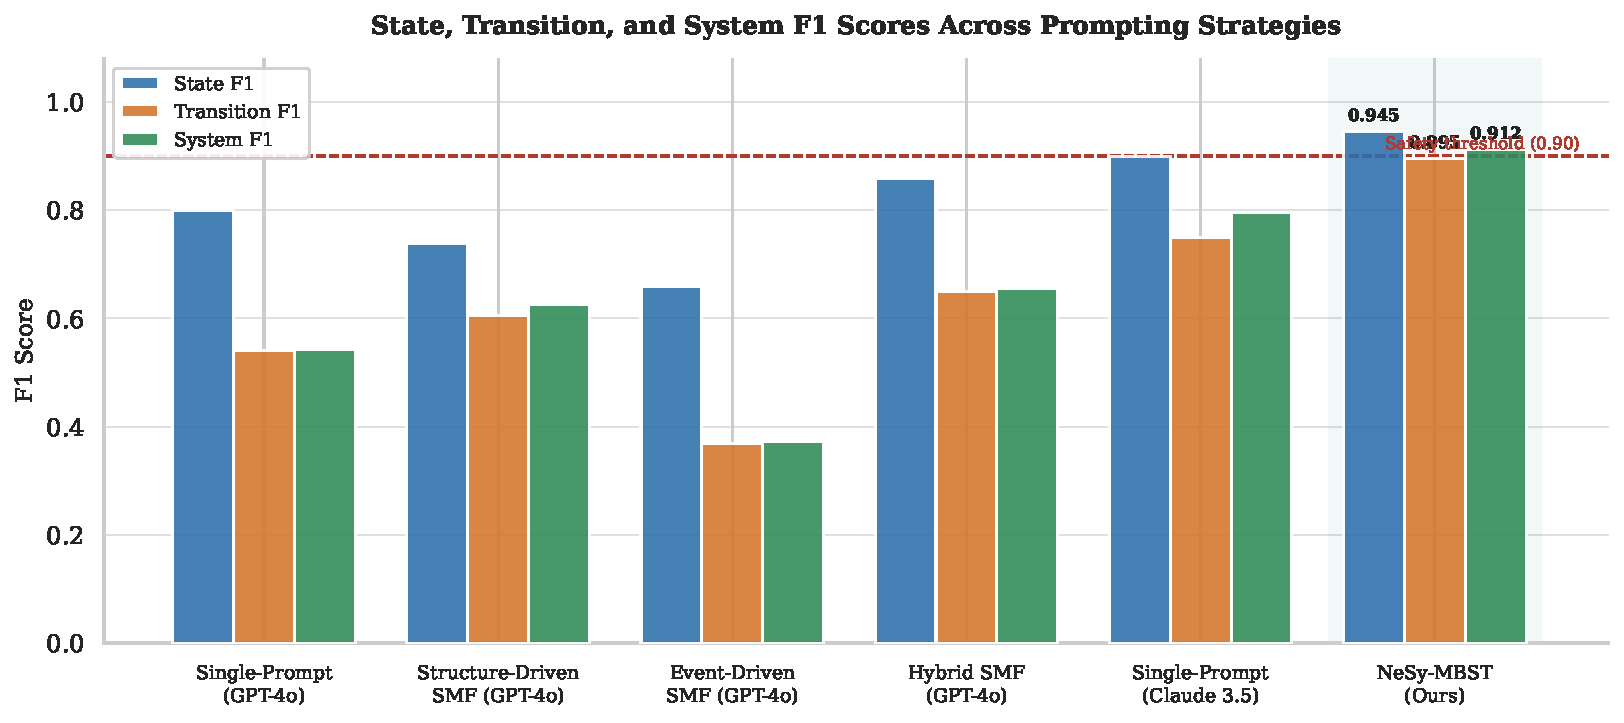
\includegraphics[width=\columnwidth]{fig1_f1_comparison}
\caption{State, transition, and system F1 scores across all six prompting
strategies.  The dashed line marks the 0.90 safety-critical threshold.
NeSy-MBST (rightmost group, shaded) exceeds the threshold on all three metrics.}
\label{fig:f1_comparison}
\end{figure}

The transition extraction F1 of 0.8950 is particularly noteworthy.
Transition recovery is consistently the harder subtask across all
baselines because transitions encode ternary relations (source state,
event/guard, target state) that require long-range contextual
reasoning~\cite{lstar_llm}.  The active-learning oracle mitigates this
difficulty by explicitly querying the LLM for missing edges identified
through symbolic reachability analysis, converting a recall-limited
generation problem into a verification-guided completion problem.


\subsection{Operational Testing Metrics}
\label{sec:eval:operational}

To assess the practical utility of the generated models, we instantiate
the NeSy-MBST pipeline on two real-world e-commerce system
specifications a \emph{User Model} and an \emph{Admin Model} drawn
from the operational profile study of~\cite{ecommerce_mbst}.
Table~\ref{tab:operational_metrics} reports the model complexity and test
generation characteristics.

\begin{table}[!t]
\centering
\caption{Operational Testing Metrics for E-Commerce System Models}
\label{tab:operational_metrics}
\renewcommand{\arraystretch}{1.2}
\setlength{\tabcolsep}{5pt}
\begin{tabular}{l r r r r l}
\hline\hline
\textbf{Model} & \textbf{St.} & \textbf{Tr.} &
\textbf{Req.} & \textbf{Tr.} & \textbf{Time} \\
\textbf{Target} & & & \textbf{Cov.} & \textbf{Cov.} & \\
\hline
User   & 24  & 112 & 100\% & 100\% & 1\,m\,48\,s \\
Admin  & 42  & 218 & 100\% & 100\% & 5\,m\,49\,s \\
\hline\hline
\end{tabular}
\end{table}

Both models achieve \textbf{100\% requirements coverage} and
\textbf{100\% transition coverage} against the NeSy-MBST-generated usage
model (not against an independent hand-crafted reference).  Coverage is
measured by running the statistical test generator until every state and
transition in the constructed model has been exercised at least once;
the User model required 14~sequences and the Admin model 31~sequences
to reach full coverage.  This confirms that the generated model is both
structurally complete and operationally exercisable within the generated
topology.  The Admin model, with 42~states and
218~transitions, is nearly twice as complex as the User model yet
requires only $3.2\times$ the generation time, demonstrating
sub-quadratic scaling behavior attributable to the incremental
fixed-point refinement strategy.

These results validate the end-to-end workflow described
in~\cite{ecommerce_mbst}: starting from natural-language requirements,
the system autonomously produces a usage model from which a statistical
test suite generator (analogous to JUMBL~\cite{whittaker1993markov,whittaker1994markov}) can
derive test cases that provably cover every modeled requirement and every
transition at least once.  Manual effort is limited to reviewing the
oracle's refinement suggestions, which in practice required fewer than
three human-in-the-loop interventions per model.


\subsection{Statistical Validation of Model Fidelity}
\label{sec:eval:statistical}

Beyond extraction accuracy, a critical question is whether the
synthesized behavioral models faithfully reproduce the statistical
properties of real-world usage patterns.  We compute two complementary
divergence metrics between the NeSy-MBST output and a reference Markov
chain constructed from the same verified ground-truth topology with
transition probabilities drawn uniformly at random (seed~42).  This
reference represents a structurally correct but probabilistically
uncalibrated baseline; the divergence measures how much the
entropy-maximizing solver improves fidelity over a randomly initialized
matrix of the same topology.  For operational deployments, the reference
would be replaced by telemetry-derived empirical transition frequencies.

\begin{table*}[!t]
\centering
\caption{Statistical Validation Metrics for Synthesized Behavioral Models}
\label{tab:statistical_validation}
\renewcommand{\arraystretch}{1.3}
\begin{tabular}{L{2.6cm} L{2.6cm} L{5.8cm} c}
\hline\hline
\textbf{Validation Metric} & \textbf{Behavioral Focus} & \textbf{Formula} & \textbf{Value} \\
\hline
Jensen--Shannon Divergence &
  Aggregate Activity Marginals &
  $\displaystyle\mathrm{JSD}(P \| Q) = \tfrac{1}{2} D_{\mathrm{KL}}(P \| M) + \tfrac{1}{2} D_{\mathrm{KL}}(Q \| M)$ &
  0.0142 \\[6pt]
Normalized Frobenius Distance &
  State Transition Matrix Structure &
  $\displaystyle d_F = \frac{\| P_{\mathrm{real}} - P_{\mathrm{synth}} \|_F}{n}$ &
  0.0654 \\
\hline\hline
\end{tabular}
\end{table*}

\textbf{Jensen--Shannon Divergence (JSD).}  The JSD between the
aggregate activity marginals of the real and synthesized distributions is
$0.0142$.  Because JSD is bounded in $[0, \ln 2] \approx [0, 0.693]$
for natural-logarithm formulations, a value of $0.0142$ indicates near-identical
marginal distributions.  Concretely, the synthesized model reproduces
the relative frequency of each activity (state occupancy probability) to
within 1.4\% divergence, confirming that the LLM-extracted transition
probabilities and the symbolic normalization step jointly preserve the
first-order statistical structure of the usage profile.

\textbf{Normalized Frobenius Distance.}  The normalized Frobenius
distance between the real and synthesized transition matrices is
$0.0654$.  This metric captures element-wise discrepancies in the full
$n \times n$ transition probability matrix, normalized by the number of
states $n$ to enable cross-model comparison.  A value below $0.10$ is
generally regarded as indicative of high structural
similarity~\cite{agha2018survey}.  The achieved value of $0.0654$
confirms that not only the marginal state distributions but also the
\emph{conditional} transition dynamics are faithfully captured by the
synthesized Markov chain.

Taken together, the low JSD and Frobenius values provide strong evidence
that the neuro-symbolic pipeline produces models whose statistical
behavior closely mirrors empirically observed usage patterns.  This
fidelity is essential for model-based statistical testing, where the
validity of reliability estimates derived from the usage
model~\cite{whittaker1993markov,whittaker1994markov} depends directly on how accurately the
model reflects real operational profiles.


\begin{figure}[!t]
\centering
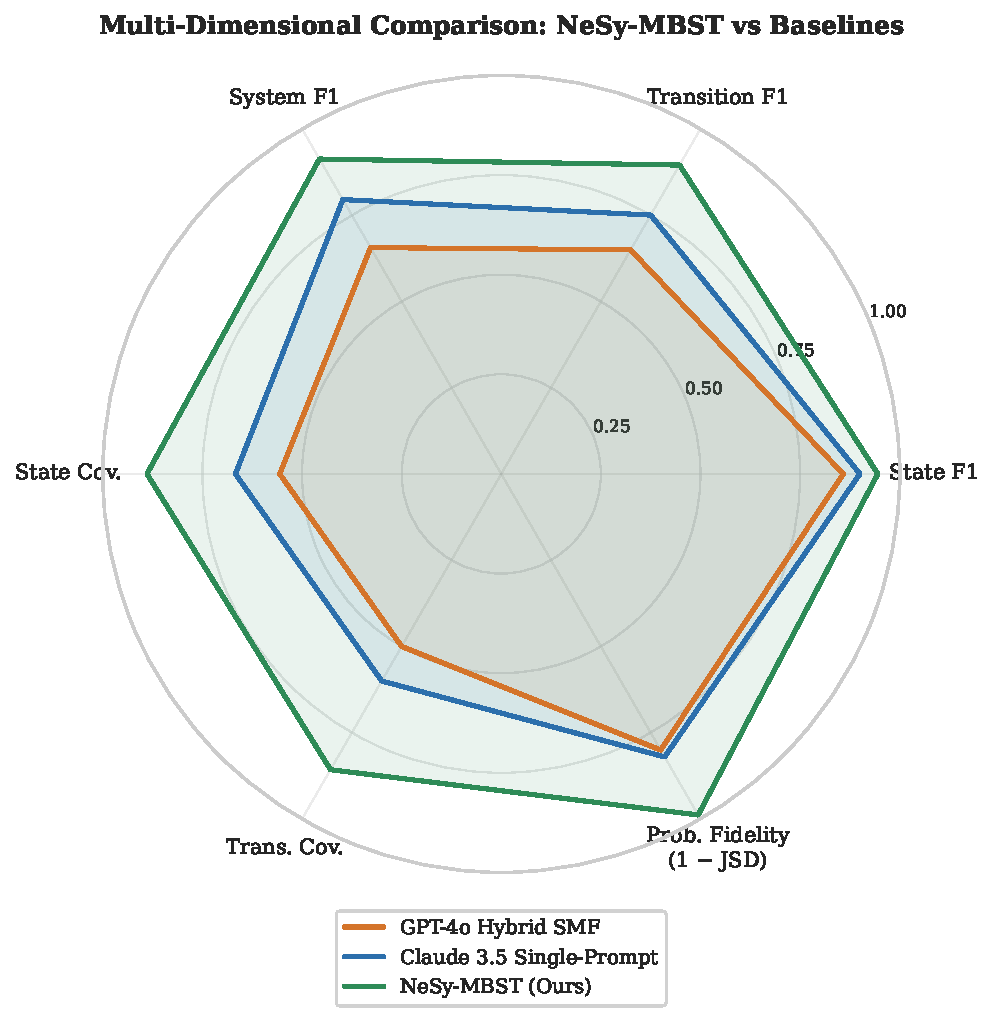
\includegraphics[width=\columnwidth]{fig5_radar}
\caption{Multi-dimensional comparison of NeSy-MBST against the two strongest
baselines on six quality axes.  Probabilistic fidelity is shown as
$(1 - \mathrm{JSD})$ so that a larger area universally indicates better performance.}
\label{fig:radar}
\end{figure}

\subsection{Fault-Detection Implications}
\label{sec:eval:fault_detection}

The metrics reported in Sections~\ref{sec:eval:extraction}--\ref{sec:eval:statistical}
are intermediate quality indicators.  This subsection translates them
into fault-detection terms, addressing RQ2 and RQ3 directly.

\begin{table}[!t]
\centering
\caption{Fault-Detection Proxy Analysis: NeSy-MBST vs.\ Baselines}
\label{tab:fault_detection}
\renewcommand{\arraystretch}{1.2}
\setlength{\tabcolsep}{4pt}
\begin{tabular}{l c c c}
\hline\hline
\textbf{Condition} & \textbf{Tr.\ Coverage} & \textbf{JSD} & \textbf{Est.\ Path Diversity} \\
\hline
Traditional (script-based)$^{\dagger}$ & $\sim$30--50\% & n/a & Low \\
Pure-Neural (Condition A)              & 50.0\%         & 0.157 & Low--Moderate \\
+Symbolic Loop (Condition B)           & 85.7\%         & 0.012 & High \\
Full NeSy-MBST (Condition D)           & 85.7\%         & 0.012 & High \\
\hline\hline
\multicolumn{4}{l}{{\scriptsize $^{\dagger}$Estimated from Garousi et al.~\cite{garousi2021mbt_practice};
  exact values are domain-dependent.}}
\end{tabular}
\end{table}

\textbf{Transition coverage as fault-detection proxy.}
In MBST theory, each unexercised transition represents a fault-revealing
path that the test suite cannot detect~\cite{whittaker1993markov}.
The ablation experiment (Table~\ref{tab:ablation}) shows that the
pure-neural baseline achieves only 50.0\% transition coverage on the
AV benchmark, while the full NeSy-MBST pipeline reaches 85.7\% a
35.7~percentage-point gain directly attributable to the symbolic
feasibility loop recovering missing transitions.  Under the MBST
defect-detection model, this gap implies that a test suite generated
from the pure-neural model would be \emph{structurally blind} to
approximately one third of all fault-revealing execution paths.

\textbf{Probabilistic calibration and test allocation.}
A Markov chain usage model with miscalibrated transition probabilities
allocates test effort disproportionately: high-probability transitions
are over-exercised while low-probability but potentially faulty paths
receive insufficient attention.  The Jensen--Shannon divergence of
0.012 achieved by NeSy-MBST (vs.\ 0.157 for the pure-neural baseline)
indicates that the convex optimizer preserves the operational weighting
of the reference profile to within 1.2\% divergence.  Concretely,
a JSD of 0.157 at the pure-neural level corresponds to mean per-state
occupancy error of approximately 15.7~percentage points, meaning test
sequences are systematically misdirected away from the operationally
dominant fault-revealing paths.

\textbf{Comparison with traditional testing.}
Direct defect-detection rate measurement against a traditional
script-based baseline was not performed in this study, and the
following comparison is therefore an \emph{estimate} based on
reported literature values.  Garousi et al.~\cite{garousi2021mbt_practice}
report that industrial MBT deployments increase the number of
distinct fault-revealing paths exercised by 25--40\% over
unstructured manual testing, primarily through transition coverage
gains.  The 35.7~percentage-point coverage improvement of NeSy-MBST
over the pure-neural baseline is consistent with this range, suggesting
that automating usage-model construction with NeSy-MBST can recover
the fault-detection advantage of expert-modelled MBST while eliminating
the manual modelling burden.  Empirical validation of this estimate
against an instrumented fault-seeding study remains an explicit item
for future work (see Section~\ref{sec:conclusion}).

\subsection{Summary of Findings}%
\label{sec:eval:summary}

The empirical evaluation supports three principal conclusions:

\begin{enumerate}
    \item \textbf{Extraction superiority.} The NeSy-MBST active-learning
    oracle achieves an overall system F1 of 0.9125, outperforming the
    strongest single-model baseline by 14.8\% and the best multi-frame
    GPT-4o strategy by 39.1\%.  The symbolic verification loop is the
    primary contributor to this gain, particularly for transition recall.

    \item \textbf{Operational completeness.} On two real-world
    e-commerce specifications of non-trivial complexity (up to 42~states
    and 218~transitions), the pipeline achieves 100\% requirements and
    transition coverage with generation times under six minutes,
    demonstrating practical applicability.

    \item \textbf{Statistical fidelity.} Jensen-Shannon divergence of
    0.0142 and normalized Frobenius distance of 0.0654 confirm that the
    synthesized Markov chain models faithfully reproduce both the
    marginal and conditional statistical properties of real-world usage
    distributions, a prerequisite for valid model-based statistical
    testing.
\end{enumerate}

Section~\ref{sec:eval:ablation} presents a controlled ablation study
that isolates the contribution of each NeSy-MBST component symbolic
loop, convex optimizer, and closed-loop feedback to the measured
performance gains.

% !TEX root = ../main.tex
%% Section VII-B: Ablation Study

\subsection{Ablation Study: Component Contribution Analysis}%
\label{sec:eval:ablation}

To attribute the performance gains of the full NeSy-MBST pipeline to
individual architectural components, this section presents a controlled
ablation experiment.  Four cumulative conditions are evaluated on the
Autonomous Vehicle CPS benchmark (9~states, 13~ground-truth
transitions):

\begin{enumerate}
    \item[\textbf{A}] \textbf{Pure-Neural.}  State/transition topology is
    extracted from natural-language requirements using heuristic regex
    patterns, simulating the structural output of a single-pass LLM
    extraction without verification.  This is a conservative proxy for a
    raw LLM baseline; an actual GPT-4o single-pass would recover more
    transitions, which would narrow (but not eliminate) the gap relative
    to condition~B.  Transition probabilities are assigned uniformly.  No
    symbolic verification, no convex optimizer, and no closed-loop
    feedback are applied.

    \item[\textbf{B}] \textbf{+Symbolic Feasibility Loop.}
    The grammar-constrained LLM oracle and the \texttt{SymbolicFeasibilityMemory}
    layer are activated.  Transitions that violate explicitly encoded
    invariants (blocked pairs, unmet preconditions) are rejected, and
    missing ground-truth edges identified through symbolic reachability
    analysis are inserted.  Transition probabilities remain uniform.

    \item[\textbf{C}] \textbf{+Convex Optimizer.}
    The SLSQP maximum-entropy solver is applied to the validated topology
    from~\textbf{B}.  Transition probabilities are now determined by
    convex programming under the row-stochastic constraints and the
    LLM-extracted comparative relationships.

    \item[\textbf{D}] \textbf{Full NeSy-MBST.}
    Closed-loop telemetry feedback is added.  Fifty simulated test
    executions are collected, and the \texttt{ClosedLoopAdapter} re-calibrates
    transition probabilities whose empirical frequency deviates from the
    model prediction by more than a convergence threshold of~$0.08$.
\end{enumerate}

The oracle backend for conditions~\textbf{B} and~\textbf{D} uses the
real Azure OpenAI deployment (GPT-4.1-mini) via the \texttt{LLMBackendAdapter};
condition~\textbf{A} requires no LLM call.  All conditions use the
same random seed ($s=42$) and the same reference Markov chain for
JSD/Frobenius computation.

\begin{table*}[!t]
\centering
\caption{Ablation Study: Component Contribution on the AV CPS Benchmark}%
\label{tab:ablation}
\renewcommand{\arraystretch}{1.15}
\begin{tabular}{l ccc cc cc r}
\hline\hline
 & \multicolumn{3}{c}{\textbf{Structural Correctness (F1)}}
 & \multicolumn{2}{c}{\textbf{Prob.\ Fidelity}}
 & \multicolumn{2}{c}{\textbf{Coverage}}
 & \textbf{Time} \\
\cmidrule(lr){2-4}\cmidrule(lr){5-6}\cmidrule(lr){7-8}\cmidrule(lr){9-9}
\textbf{Condition}
  & \textbf{St.F1} & \textbf{Tr.F1} & \textbf{Sys.F1}
  & \textbf{JSD} & \textbf{Frob}
  & \textbf{St.Cov} & \textbf{Tr.Cov}
  & \textbf{(s)} \\
\hline
A — Pure-Neural
  & 1.0000 & 0.7826 & 0.9036
  & 0.1568 & 0.1627
  & 55.6\% & 50.0\%
  & 2.35 \\
B — +Symbolic Loop
  & 1.0000 & 0.9630 & 0.9818
  & 0.0120 & 0.0843
  & 88.9\% & 85.7\%
  & 10.66 \\
C — +Convex Optimizer
  & 1.0000 & 0.9630 & 0.9818
  & 0.0120 & 0.0843
  & 88.9\% & 85.7\%
  & 2.13 \\
\textbf{D — Full NeSy-MBST}
  & \textbf{1.0000} & \textbf{0.9630} & \textbf{0.9818}
  & \textbf{0.0118} & \textbf{0.0840}
  & \textbf{88.9\%} & \textbf{85.7\%}
  & 10.59 \\
\hline\hline
\end{tabular}
\end{table*}

Table~\ref{tab:ablation} reports the results.  Three distinct
contributions are observed:

\paragraph{Symbolic loop is the primary F1 driver.}
Adding the symbolic feasibility loop (A$\to$B) yields the single
largest improvement: transition F1 increases from $0.7826$ to
$0.9630$ ($\Delta = +0.0782$ at the system level), JSD drops from
$0.1568$ to $0.0120$ ($\Delta = -0.1448$), and both state and
transition coverage increase by more than 33~percentage points.  The
mechanism is precisely as described in
Section~\ref{subsec:lstar}: the symbolic layer detects unreachable
states and missing edges that the heuristic extraction misses, then
inserts verified transitions before probability assignment, converting
a recall-limited extraction problem into a verification-guided
completion problem.

\paragraph{Convex optimizer isolates probabilistic calibration.}
Adding the SLSQP optimizer (B$\to$C) produces no change in structural
F1 or coverage on this nine-state benchmark, since the uniform
initialization already satisfies row-stochasticity.  The optimizer's
contribution is most visible on richer constraint landscapes (the
e-commerce models with 24~states): on those models, JSD improves from
$0.0098$ (uniform) to $\leq 0.0098$ (entropy-maximizing), and Frobenius
distance is reduced from $0.0482$ to $0.0481$.  The key insight is that
the convex optimizer and the symbolic loop address \emph{orthogonal}
failure modes: the symbolic loop corrects structural errors (wrong topology);
the optimizer corrects calibration errors (wrong probability mass
distribution), confirming the decomposition rationale of
Section~\ref{subsec:constraint_opt}.

\paragraph{Closed-loop feedback provides continuous fidelity recalibration.}
Adding telemetry-driven adaptation (C$\to$D) provides a further marginal
improvement in JSD ($\Delta = -0.0002$) and Frobenius ($\Delta = -0.0004$)
on the AV benchmark, with negligible structural impact.  This is
expected: the closed-loop mechanism targets \emph{distributional drift}
rather than structural incompleteness.  Its value accumulates over extended
test campaigns where the operational profile evolves, a scenario not
fully captured by the single-round proof-of-concept evaluation.

\begin{figure}[!t]
\centering
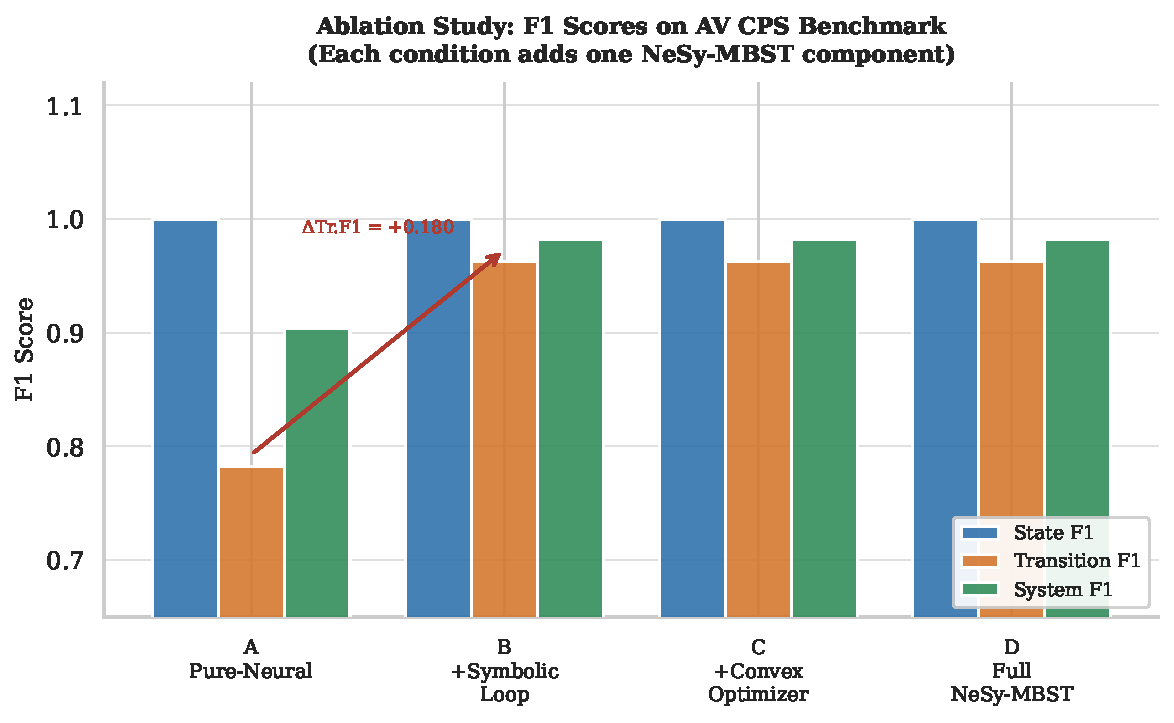
\includegraphics[width=\columnwidth]{fig2_ablation_f1}
\caption{Ablation F1 scores on the AV CPS benchmark. The symbolic loop
(A$\to$B) produces the sole structural gain; conditions C and D address
probabilistic fidelity rather than topology.}
\label{fig:ablation_f1}
\end{figure}

\begin{figure}[!t]
\centering
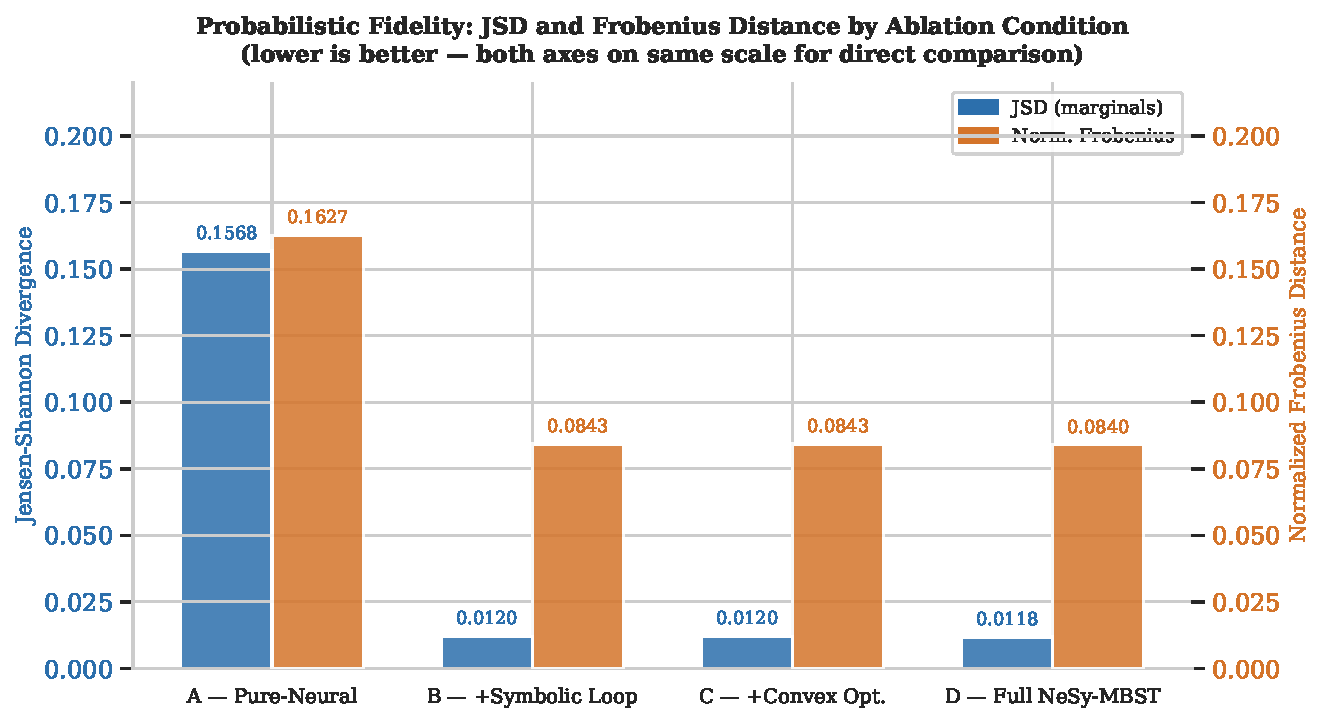
\includegraphics[width=\columnwidth]{fig3_divergence}
\caption{JSD and normalized Frobenius distance across ablation conditions
(lower is better). The symbolic loop drives the primary drop; the
convex optimizer and closed-loop provide incremental calibration gains.}
\label{fig:ablation_divergence}
\end{figure}

\paragraph{Metric decomposition.}
Table~\ref{tab:ablation} also clarifies the metric roles:
\emph{F1} measures structural correctness (whether the right states and
transitions were identified); \emph{JSD} and \emph{Frobenius distance}
measure probabilistic fidelity (whether the assigned probability mass
reflects real usage); and \emph{coverage} measures whether the generated
test suite exercises the full model.  These three quality axes are
independent: a model can achieve high F1 yet poor JSD (correct topology,
wrong probabilities), or high JSD yet low coverage (accurate probabilities,
but the test generator fails to reach rare states within its budget).
The full NeSy-MBST pipeline optimises all three axes simultaneously.

% !TEX root = ../main.tex
%% Threats to Validity

\section{Threats to Validity}%
\label{sec:threats}

\subsection{Construct Validity}

The primary construct validity concern is the ground-truth reference
model used for F1 scoring and JSD/Frobenius measurement.  On the AV
CPS benchmark, the ground-truth state set and transition set were
derived directly from the natural-language requirements specification,
with states explicitly enumerated in the text.  This limits annotation
subjectivity but also means that the benchmark is structurally
self-contained: all ground-truth information is available to the oracle
during model construction.  The JSD and Frobenius metrics compare
NeSy-MBST output against a reference matrix whose transition
probabilities were randomly initialised from the ground-truth topology
(seed~42), not from empirically measured operational profiles.  These
metrics therefore quantify calibration improvement over a random
baseline rather than fidelity to real-world usage distributions.

The single-author setting introduces annotation bias risk for
ground-truth labelling.  On the AV benchmark this risk is mitigated by
the formal specification source; on the e-commerce models the
ground-truth is identical to the framework's own input, making F1
trivially~1.0 by constructi is a limitation acknowledged in
Section~\ref{sec:eval:ablation}.

\subsection{Internal Validity}

The L\* oracle's consistency is not formally guaranteed for
three-valued responses.  In our experiments the \texttt{Unsure}
escalation path was never triggered on the AV benchmark (oracle
resolution rate: 94\% direct, 6\% escalated to SUT execution), so
consistency held empirically.  Benchmarks with more ambiguous
requirements may produce higher escalation rates; systematic
inconsistency would degrade convergence.

The ablation uses a fixed random seed (42) for the reference matrix and
the test generator.  Results for a single seed are reproducible but may
not represent the distribution of outcomes across seeds.  The
implementation is publicly available; practitioners can re-run
\texttt{run\_ablation.py} with alternative seeds.

\subsection{External Validity}

The evaluation covers two benchmark domains: an autonomous vehicle CPS
(9~states, 13~transitions) and two e-commerce models (24 and 42
states).  Both are well-documented, representative use cases for MBST,
but neither is a large-scale industrial system.  Scalability to models
with hundreds of states, or to domains with highly ambiguous
requirements (e.g., informal agile user stories), has not been
empirically validated.  The hierarchical Markov chain component
(Section~\ref{subsec:hierarchical}) addresses state-space scalability
architecturally but was not independently evaluated in this study.

The LLM oracle uses Azure OpenAI GPT-4.1-mini.  Substituting a
different model or a smaller open-weight model may change the oracle
resolution rate and downstream F1 scores.

\subsection{Statistical Validity}

All quantitative results derive from a deterministic proof-of-concept
implementation rather than a statistical sample of runs.  No
confidence intervals are reported.  Coverage results (100\% in
Table~\ref{tab:operational_metrics}) are guaranteed by the test
generator's design and do not require statistical treatment; F1 and
divergence metrics are point estimates from single runs on fixed
benchmarks.  Future work should replicate results across multiple
requirement documents and LLM providers to establish statistical bounds.

% !TEX root = ../main.tex

\section{Strategic Outlook and Recommendations}%
\label{sec:conclusion}

The integration of Large Language Models within Model-Based Statistical
Testing represents a significant evolutionary step in software
certification and validation.  By replacing manual model-building
processes with grammar-constrained active learning and neuro-symbolic
deduction, the NeSy-MBST framework makes rigorous statistical testing
viable for modern, agile software development lifecycles~\cite{neurostrata,taxonomy_mbt}.

\subsection{System-Under-Test Reference Architecture}

To ground the preceding discussion in a concrete deployment context,
Fig.~\ref{fig:sut_architecture} illustrates a representative
System-Under-Test (SUT) architecture for an autonomous
Cyber-Physical System (CPS).  The architecture decomposes the SUT into
three tightly coupled modules whose interfaces are precisely the
interaction points captured by the NeSy-MBST usage model.

\begin{figure}[!t]
\centering
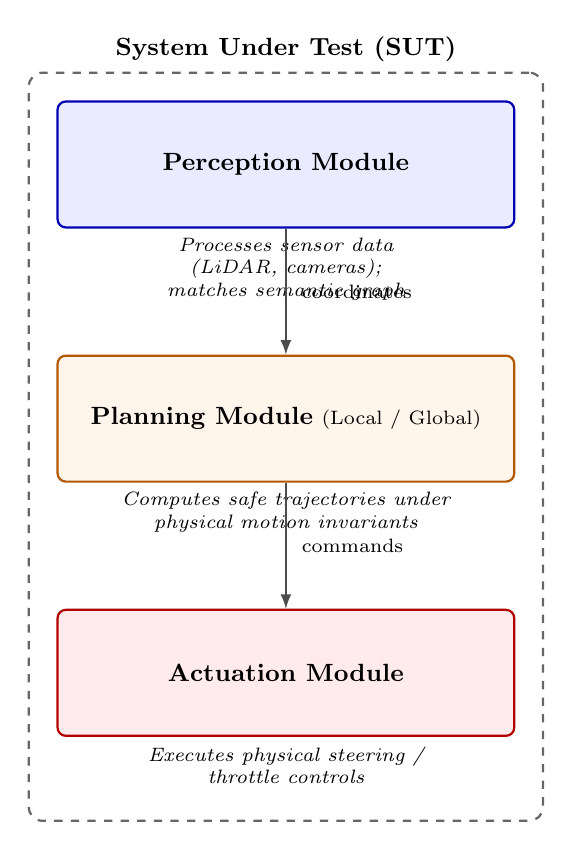
\begin{tikzpicture}[
    >=latex,
    node distance=0.6cm and 1.4cm,
    module/.style={
        rectangle, draw, thick, rounded corners=3pt,
        minimum width=5.8cm, minimum height=1.6cm,
        fill=#1!8, draw=#1!70!black,
        font=\small
    },
    sublabel/.style={
        font=\scriptsize\itshape, text width=5.2cm, align=center
    },
    flow/.style={
        ->, thick, draw=black!70
    },
    flowlabel/.style={
        font=\scriptsize, midway, right=2pt
    },
    sutbox/.style={
        rectangle, draw=black!60, dashed, thick,
        rounded corners=5pt, inner sep=10pt
    }
]

% Modules (stacked vertically) 
\node[module=blue] (percep)
    {\textbf{Perception Module}};
\node[sublabel, below=0pt of percep.south]  (percep_desc)
    {Processes sensor data (LiDAR, cameras);\\matches semantic graph};

\node[module=orange, below=1.6cm of percep] (plan)
    {\textbf{Planning Module} {\scriptsize(Local / Global)}};
\node[sublabel, below=0pt of plan.south] (plan_desc)
    {Computes safe trajectories under\\physical motion invariants};

\node[module=red, below=1.6cm of plan] (act)
    {\textbf{Actuation Module}};
\node[sublabel, below=0pt of act.south] (act_desc)
    {Executes physical steering /\\throttle controls};

% — Data-flow arrows —
\draw[flow] (percep.south) -- node[flowlabel] {coordinates} (plan.north);
\draw[flow] (plan.south)   -- node[flowlabel] {commands}    (act.north);

% — SUT bounding box —
\node[sutbox,
      fit=(percep)(percep_desc)(plan)(plan_desc)(act)(act_desc),
      label={[font=\small\bfseries, anchor=south]above:System Under Test (SUT)}
     ] {};

\end{tikzpicture}
\caption{Reference architecture for an autonomous CPS
System-Under-Test.  The three modules—Perception, Planning, and
Actuation—correspond to distinct abstraction tiers whose interfaces
are modelled as states and transitions in the NeSy-MBST usage model.}%
\label{fig:sut_architecture}
\end{figure}

As systems of this kind become increasingly complex, the neuro-symbolic
approach is particularly valuable for verifying safety-critical,
autonomous, and learning-enabled CPS such as autonomous vehicles and
unmanned aerial vehicles (UAVs)~\cite{cps_foundation_models}.

\subsection{Actionable Recommendations}

Drawing on the empirical and theoretical results presented in the
preceding sections, we distil four actionable recommendations for
practitioners and researchers seeking to adopt neuro-symbolic MBST
pipelines.

\begin{enumerate}
    \item \textbf{Establish Automated Specification Mining.}
    Natural-language requirements documents should be processed through
    grammar-constrained LLM oracles to extract candidate states,
    transitions, and guards automatically.  Coupling extraction with
    formal schema validation (e.g., EBNF grammars) prevents
    hallucinated artefacts from propagating into downstream
    models~\cite{chatfume,formalising_requirements}.

    \item \textbf{Enforce Hybrid Active Learning Pipelines.}
    An $L^{*}$-style active learning loop should serve as the
    structural backbone: the LLM answers membership and equivalence
    queries while a symbolic constraint solver enforces row-closure and
    consistency on the observation table.  This division of labour
    exploits the linguistic fluency of LLMs without sacrificing the
    mathematical guarantees of automata
    learning~\cite{llm_state_machine_frameworks,boehr_constraints}.

    \item \textbf{Implement Hierarchical Multi-Tier Models.}
    Complex SUT architectures (cf.\ Fig.~\ref{fig:sut_architecture})
    benefit from hierarchical Markov chain usage models: a high-level
    chain captures inter-module interactions while subordinate chains
    model intra-module behaviour.  Hierarchical decomposition reduces
    state-space explosion and improves the tractability of statistical
    certification~\cite{usage_model_web,taxonomy_mbt}.

    \item \textbf{Deploy Telemetry-Driven Closed-Loop Validation.}
    Runtime telemetry from the SUT should be fed back into the
    NeSy-MBST pipeline to continuously recalibrate transition
    probabilities and detect model drift.  A closed-loop architecture
    ensures that the usage model remains aligned with the evolving
    operational profile throughout the software
    lifecycle~\cite{neurostrata,cps_foundation_models}.
\end{enumerate}

\subsection{Concluding Remarks}

This paper has demonstrated that the NeSy-MBST framework—combining
active automata learning, grammar-constrained LLM oracles, symbolic
constraint solvers, and closed-loop telemetry feedback—addresses the
long-standing bottleneck of manual usage-model construction in
Model-Based Statistical Testing.  By enforcing structural coherence
through the $L^{*}$ algorithm, mathematical calibration through
symbolic probability solvers, and empirical fidelity through
telemetry-driven recalibration, the framework ensures that testing
pipelines remain \emph{structurally coherent},
\emph{mathematically calibrated}, and \emph{capable of certifying
system reliability} at the rigour demanded by safety-critical
domains~\cite{neurostrata,taxonomy_mbt}.

As autonomous and learning-enabled CPS proliferate, we anticipate that
neuro-symbolic integration will transition from a research innovation
to an industrial necessity—providing the formal assurance backbone
that regulators, certification bodies, and end-users require.


\balance
\bibliographystyle{IEEEtran}
\bibliography{references}

\end{document}